\chapter{Реализация программного обеспечения} \label{ch:ch3}
\section{Топология blockchain сети} \label{sec:ch3:sec1}
Для развертки сети для разработки используются утилиты командной строки, входящие в дистрибутив Hyperledger Fabric. Большинство из них читают некоторую конфигурацию и запускают соответствующее ПО в контейнерах, образуя узлы сети. Топология сети для разработки представлена на рисунке \ref{fig:network-topology}. Она состоит из 2 обычных узлов и 1 узла сервисной службы. Обычные узлы  владеют своей собственной базой данных Coachdb, хранящей локальную копию блокчейна.

\begin{figure}[ht]
	\centering
	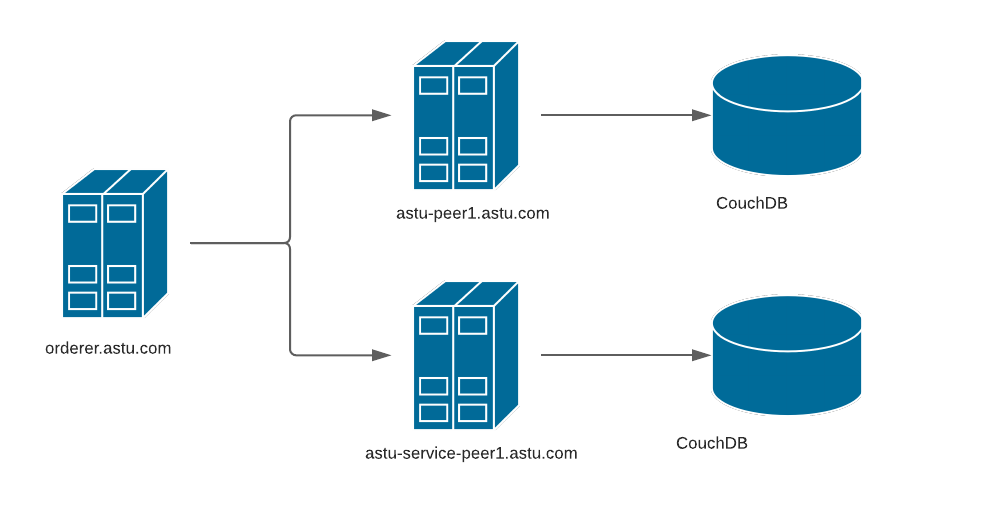
\includegraphics [scale=1.0] {network-topology}
	\caption{Топология сети Fabric, участвовавшая в разработке.}
	\label{fig:network-topology}
\end{figure}

Также существуют конфигурации для подключения к удаленной среде Fabric. В них описывается структура сети, такие элементы, как каналы, узлы, огранизации и т.д. Предназначение этих конфигураций заключается в описании существующей сети Fabric SDK для успешной её работы. Пример конфигурации используемой сервером для подключения к сети, предназначенной для разработки и отладки смарт контрактов представлен на рисунке \ref{fig:dev-network-connection}.

\begin{figure}[H]
	\centering
	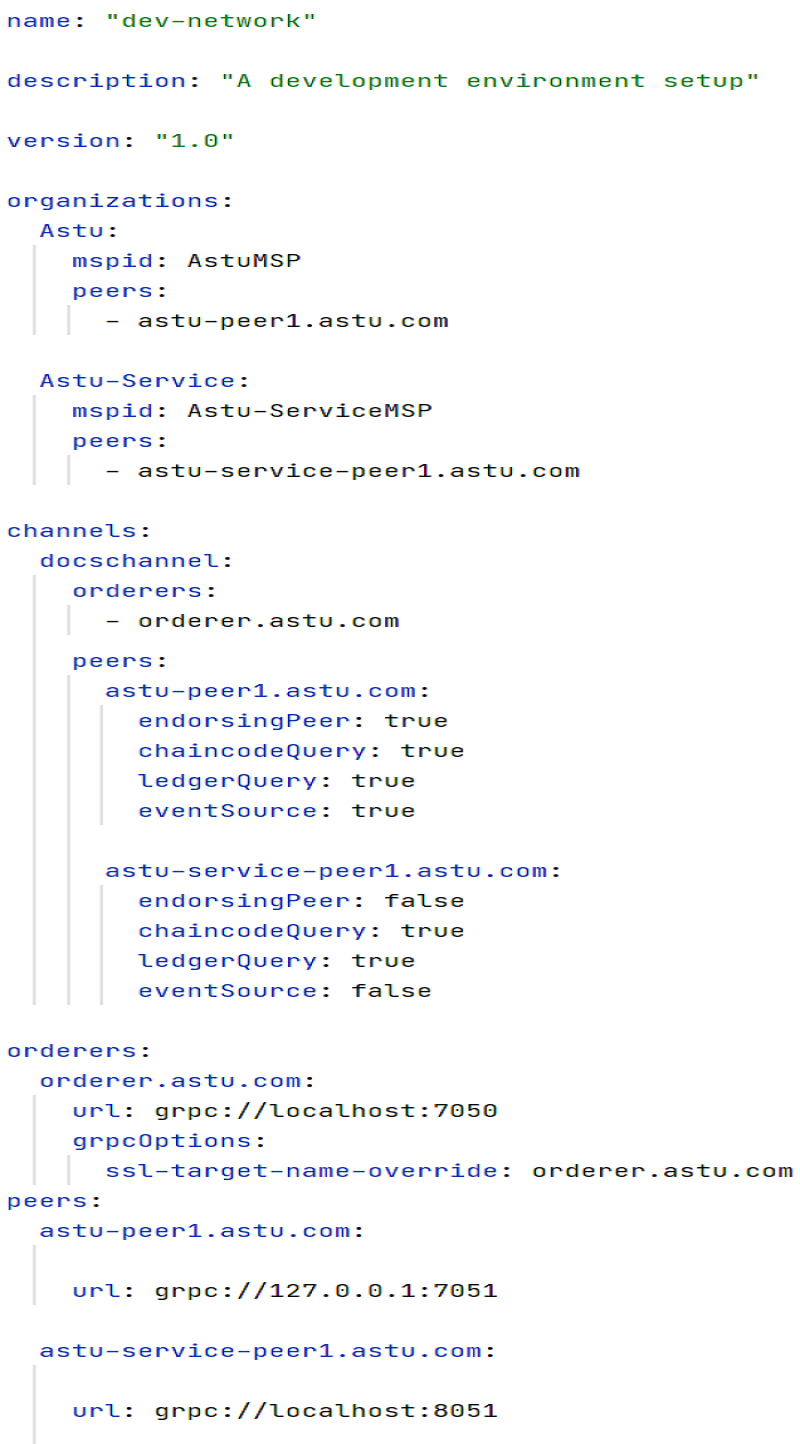
\includegraphics [scale=0.8] {dev-network-connection}
	\caption{Конфигурация подключения к сети Fabric.}
	\label{fig:dev-network-connection}
\end{figure}

\section{Серверная часть} \label{sec:ch3:sec2}

Серверная часть документооборота написана на платформе Node.js с использованием языка JavaScript. Благодаря этой платформе скриптовый язык  JavaScript можно использовать в качестве универсального языка программирования. На рисунке \ref{fig:server-architecture} представлена архитектура серверной части.

\begin{figure}[ht]
	\centering
	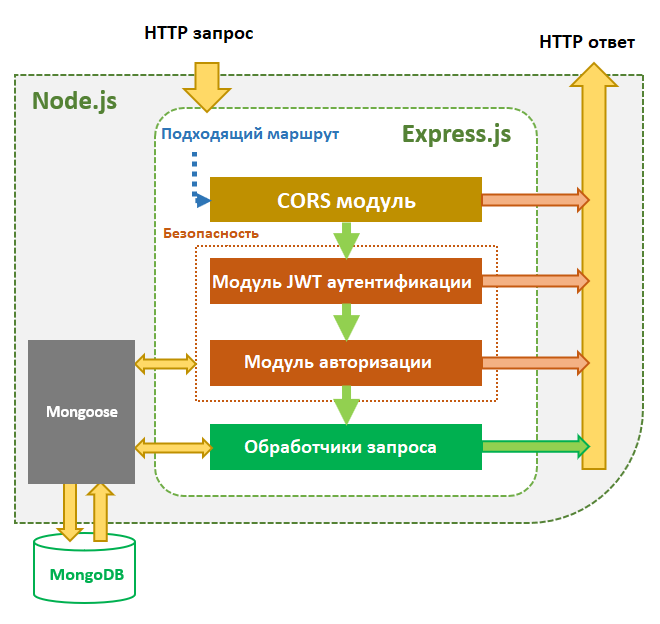
\includegraphics [scale=1.0] {node-js-rus}
	\caption{Архитектура серверной части.}
	\label{fig:server-architecture}
\end{figure}

Сервер предоставляет внешние API, которые могут быть вызваны клиентскими приложениями. Логику API реализуют контроллеры из рисунка \ref{fig:server-architecture}.  

Логически API поделены на 3 группы:
\begin{itemize}
	\item \textbf{Аутентификации и авторизации (АА)} - \textit{/api/auth/**}  - используются для регистрации и авторизации участников документооборота;
	\item \textbf{Сервиса} - \textit{/api/service/**} - используются для представления клиентам информации о структуре возможных документов;
	\item \textbf{Смарт контрактов} - \textit{/api/chaincode/**} - используются для обращение к среде выполнения Fabric с целью исполнения смарт контрактов посредством Fabric SDK.
\end{itemize}

\subsection{Поддержка документов разных типов} \label{subsec:ch3/sec1/subsec1}

Почти любой документ должен соответствовать некоторым стандартам и положениям. Из этого вытекает, то, что структура некоторых документов будет повторяться в зависимости от его типа. Для того чтобы пользователи разработанной системы не были вынуждены производить рутинное написание одних и тех же текстовых содержаний документа (отличающимися лишь некоторыми данными), система документооборота должна поддерживать типизацию документов, которая заключается в хранении атрибутов документа и динамической генерации текстовой составляющей документа. Реализован данный механизм следующим образом: в файловой системе сервера хранятся конфигурации формы для ввода атрибутов текста в формате json, которые подвергается разбору со стороны клиентского приложения и используются им для динамического построения форм ввода атрибутов документов. Пример такой конфигурации для документов типа General представлен в листинге \ref{lst:form-config-general}.

\begin{lstlisting}[caption={Json-конфигурация формы по извлечению аттрибутов документа типа General},label={lst:form-config-general},language=JavaScript]
[
{
	"_id": "title_hint",
	"text": "Название документа",
	"type": 1
},
{
	"_id": "title",
	"is_required": true,
	"hint": "Название документа",
	"type": 2
},
{
	"_id": "content_hint",
	"text": "Текст документа",
	"type": 1
},
{
	"_id": "content",
	"is_required": true,
	"max_length": 7,
	"hint": "Текст документа",
	"type": 12
},
{
	"_id": "signs",
	"hint": "Выберите подписи",
	"text": "Подписи",
	"list": [
	
	],
	"type": 11
},
{
	"_id": "submit",
	"text": "Ок",
	"type": 10
}
]
\end{lstlisting}

Как видно из листинга \ref{lst:form-config-general}, конфигурация формы представляет из себя json массив объектов, служащих для описания элементов интерфейса формы, посредством которой происходит ввод атрибутов документа. Среди атрибутов есть как не уникальные (такие, например, как название и список подписантов) как и уникальные для некоторого типа (например, список студентов и тип практики, если речь идет о приказе о направлении на практику). В листинге \ref{lst:form-config-general} уникальным для своего типа является атрибут content. Он представляет из себя текст документа, который может быть абсолютно любым, данный тип существует для создания неизвестных до некоторого момента типов документов, либо с еще не зафиксированной структурой. Впоследствии такой документ можно будет типизировать в разработанной системе без особых усилий со стороны разработчика. Необходимо будет добавить конфигурацию формы, разработав структуру его атрибутов, и шаблон текстовой составляющей документа. Шаблон представляет из себя текстовый файл с внедренными в него участками JavaScript кода, оперирующего атрибутами документа. При запросе документа на сервере производится замена всех участков кода на значения выполненных выражений. Пример такого шаблона приведен на рисунке \ref{fig:doc-template-practice-permission}.
\begin{figure}[H]
	\centering
	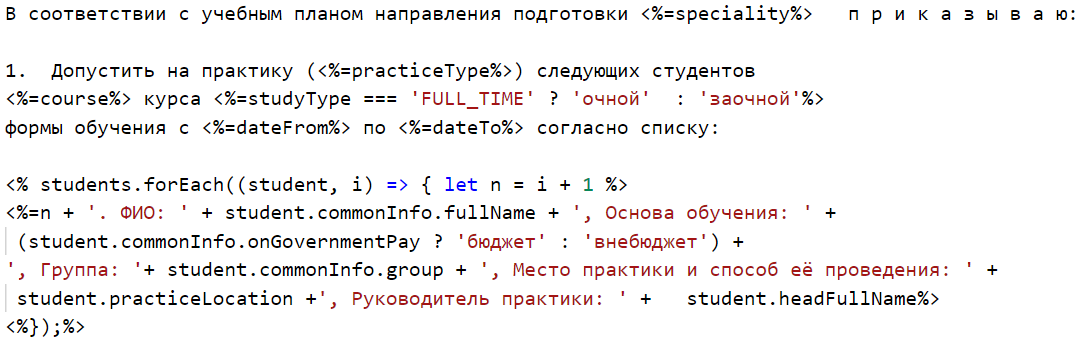
\includegraphics [scale=0.9] {doc-template-practice-permission}
	\caption{Шаблон текстовой составляющей документа типа PracticePermission}
	\label{fig:doc-template-practice-permission}
\end{figure}

Также стоит отметить, что при реализованном устройстве представления текстового содержимого документа, один и тот же документ может быть предоставлен пользователю по разному, для этого достаточно поменять (или изменить) шаблон типа документа. А также, разделение сущности документа на представление и хранимые атрибуты делает удобным восприятие документов различными системами, помимо разработанного клиентского приложения. К таким системам можно отнести дашборды и обозреватели документооборота, которые могут быть интегрированы с разработанным СЭД.
 
\subsection{Описание методов веб-API} \label{subsec:ch3/sec1/subsec2}

В таблице~\ref{tab:apis} представлены маршруты внешних АПИ серверной части приложения, сгруппированные по назначению, как упоминалось в \ref{sec:ch3:sec1}.
\begin{longtable} {| p{8.3cm} | p{8.35cm}l |}
	\caption{Список API серверной части}
	\label{tab:apis}\\
	\hline
	\centering Наименование &  \centering Описание & \\
	\hline
	\multicolumn{2}{|c}{\textbf{API сервиса}} & \\
	\hline
	\endfirsthead
	\caption*{Продолжение таблицы \ref{tab:apis}}\\
	\hline
	\centering Наименование &  \centering Описание & \\
	\hline
	\endhead
	\hline
	\endfoot
	/api/service/getFormConfig (POST) & Получение конфигурации формы для документа определенного типа. &\\
	\hline
	/api/service/getDocTypes (POST) & Получение поддерживаемых типов документов &\\
	\hline
	\multicolumn{2}{|c}{\textbf{API аутентификации и авторизации}} & \\
	\hline
	/api/auth/signIn (POST) & Вход в систему участника документооброта по логину и паролю. &\\
	\hline
	\multicolumn{2}{|c}{\textbf{API смарт контрактов}} & \\
	\hline
	/api/chaincode/newDoc (POST) & Создание нового документа в системе документооброта. &\\
	\hline
	/api/chaincode/getDocs (POST) &Получение списка документов для некоторой группы пользователей &\\
	\hline
	/api/chaincode/changeDoc (POST) & Изменение состояния (одобрение, отклонение, редактирование) существующего документа &\\
\end{longtable}

На рисунках \ref{fig:api-first}-\ref{fig:api-last} приведены диаграммы, описывающие API из таблицы \ref{tab:apis}.

\begin{figure}[H]
	\centering
	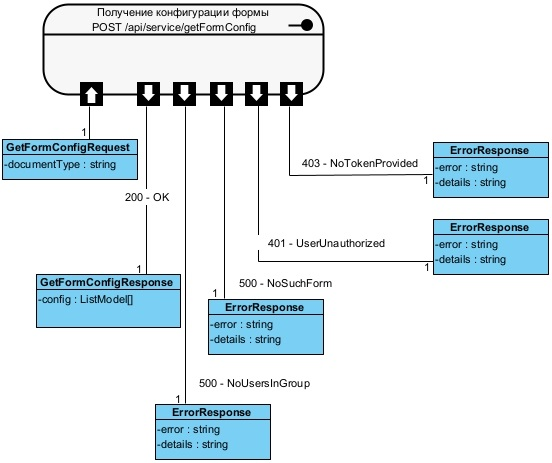
\includegraphics [scale=1.0] {api-getFormConfig}
	\caption{Диаграмма /api/service/getFormConfig.}
	\label{fig:api-first}
\end{figure}

\begin{figure}[H]
	\centering
	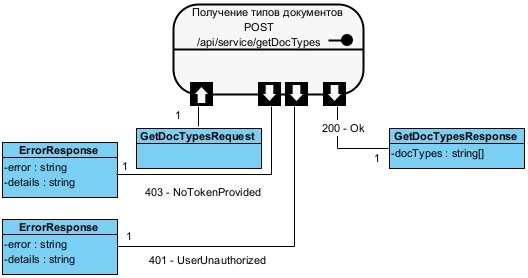
\includegraphics [scale=1.0] {api-getDocTypes}
	\caption{Диаграмма /api/service/getDocTypes.}
	\label{fig:api-getDocTypes}
\end{figure}

\begin{figure}[H]
	\centering
	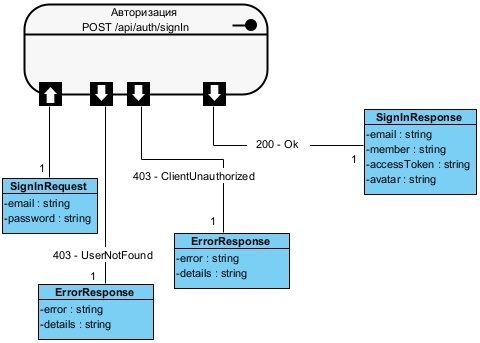
\includegraphics [scale=1.0] {api-signIn}
	\caption{Диаграмма /api/service/getFormConfig.}
	\label{fig:api-signIn}
\end{figure}

\begin{figure}[H]
	\centering
	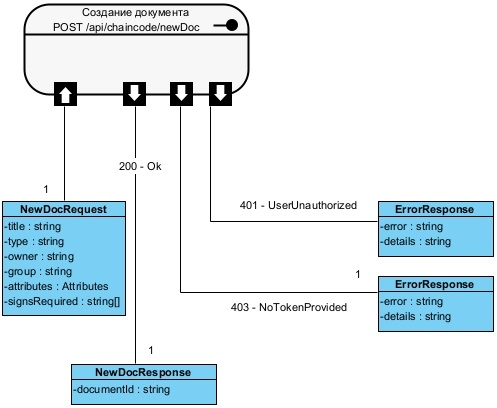
\includegraphics [scale=1.0] {api-newDoc}
	\caption{Диаграмма /api/service/getFormConfig.}
	\label{fig:api-newDoc}
\end{figure}

\begin{figure}[H]
	\centering
	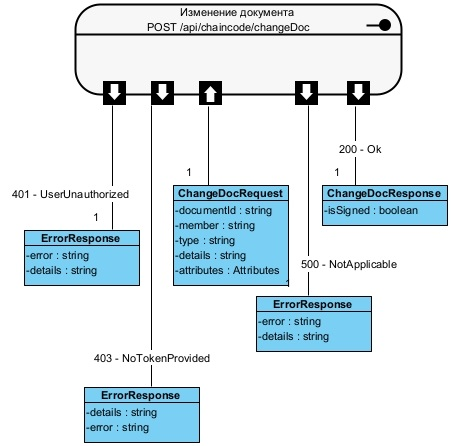
\includegraphics [scale=1.0] {api-changeDoc}
	\caption{Диаграмма /api/service/getFormConfig.}
	\label{fig:api-changeDoc}
\end{figure}

\begin{figure}[H]
	\centering
	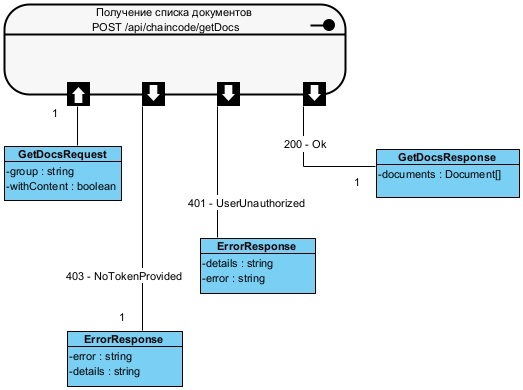
\includegraphics [scale=1.0] {api-getDocs}
	\caption{Диаграмма /api/chaincode/getDocs.}
	\label{fig:api-last}
\end{figure}

\section{Клиентская часть} \label{sec:ch3:sec3}

При реализации клиентского приложения использовался шаблон проектирования архитектуры мобильных приложений MVVVM (Model-View-ViewModel) \cite{anrdoid}.

\begin{figure}[ht]
	\centering
	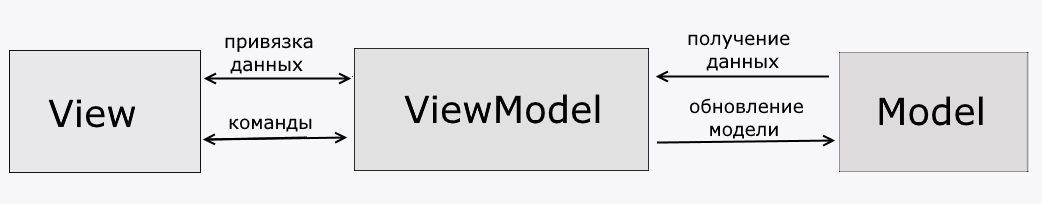
\includegraphics [scale=0.4] {mvvm}
	\caption{Архитектура MVVM.}
	\label{fig:mvvm}
\end{figure}

Такой подход к проектированию архитектуры позволяет разделить представление данных от их модели, что облегчает разработку приложения. А также он позволяет эффективно работать со <<связыванием данных>>, осуществляющее двусторонние связывание данных с визуальными элементами интерфейса. Эта механика, в свою очередь, основана на шаблоне проектирования <<Наблюдатель>>, т.е. при изменение состояние какого либо объекта происходит вызов функций обратного вызова подписчиков. В нашем случае интерфейс и данные являются подписчиками и наблюдателями друг друга.

\subsection{Диаграммы классов} \label{subsec:ch3/sec2/subsec2}
На рисунке \ref{fig:MiddlewareClientNoPackage} изображена диаграмма классов модуля-потребителя API. На рисунке \ref{fig:UiNoPackageRotated} изображена диаграмма классов, отвечающих за работу графического интерфейса.
\begin{figure}[H]
	\centering
	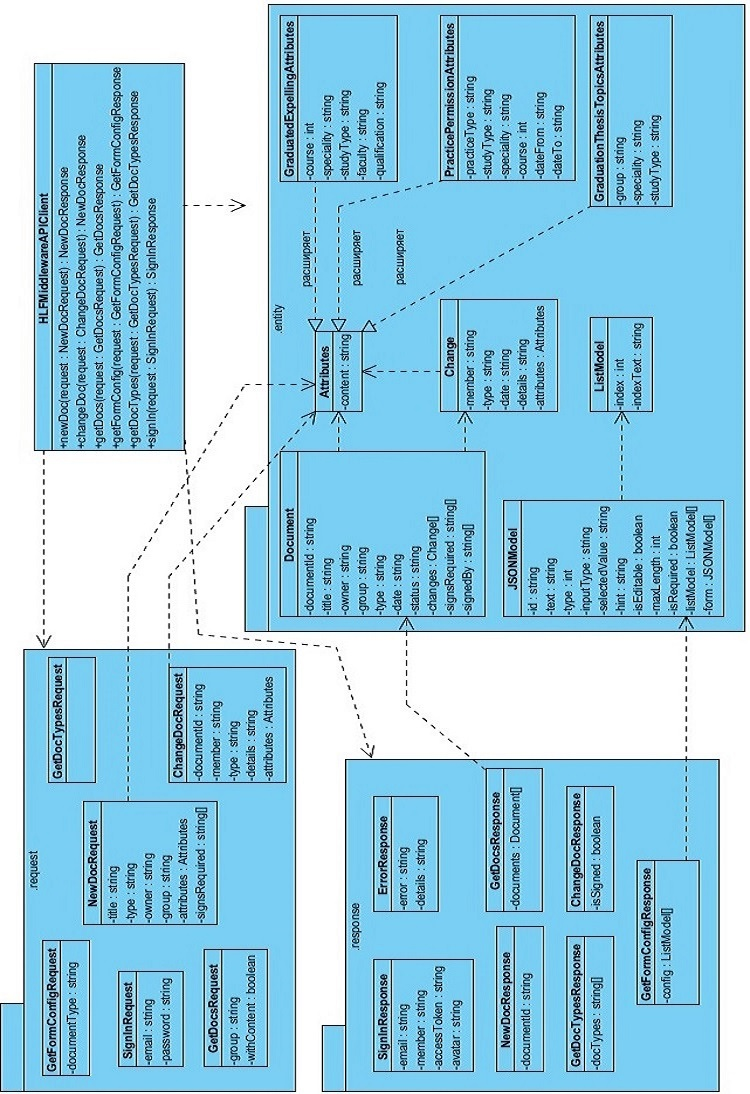
\includegraphics [scale=1.0] {MiddlewareClientNoPackageRotated}
	\caption{Диаграмма классов потребителя API связующего ПО.}
	\label{fig:MiddlewareClientNoPackage}
\end{figure}

\begin{figure}[H]
	\centering
	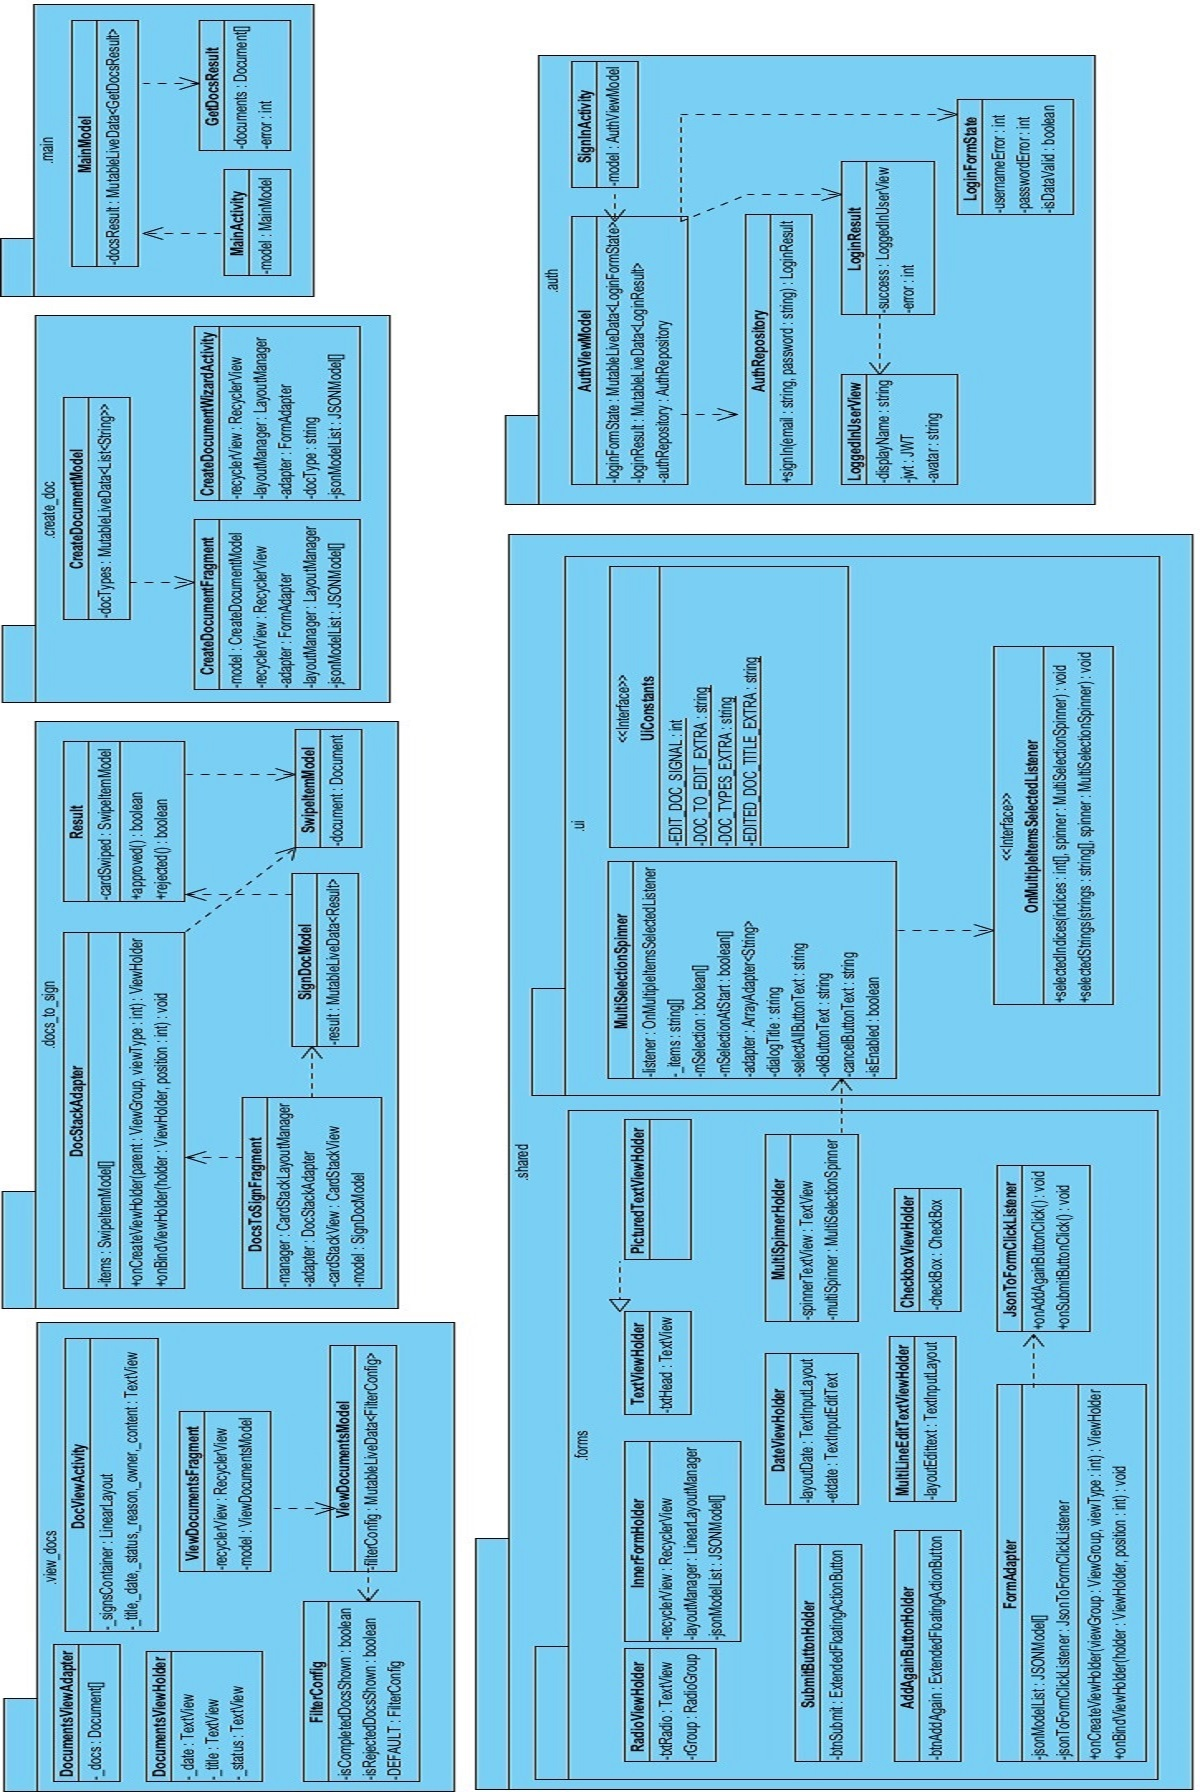
\includegraphics [scale=0.65] {UiNoPackageRotated}
	\caption{Диаграмма классов пользовательского графического интерфейса.}
	\label{fig:UiNoPackageRotated}
\end{figure}


\subsection{Пользовательский интерфейс} \label{subsec:ch3/sec2/subsec3}
Описанным в \ref{subsec:ch2/sec3/subsec4/subsubsec1} сценариям сопутствует использование графического интерфейса программы показанного на рисунках \ref{fig:ui-first} - \ref{fig:ui-last}

\begin{figure}[ht]
	\centering
	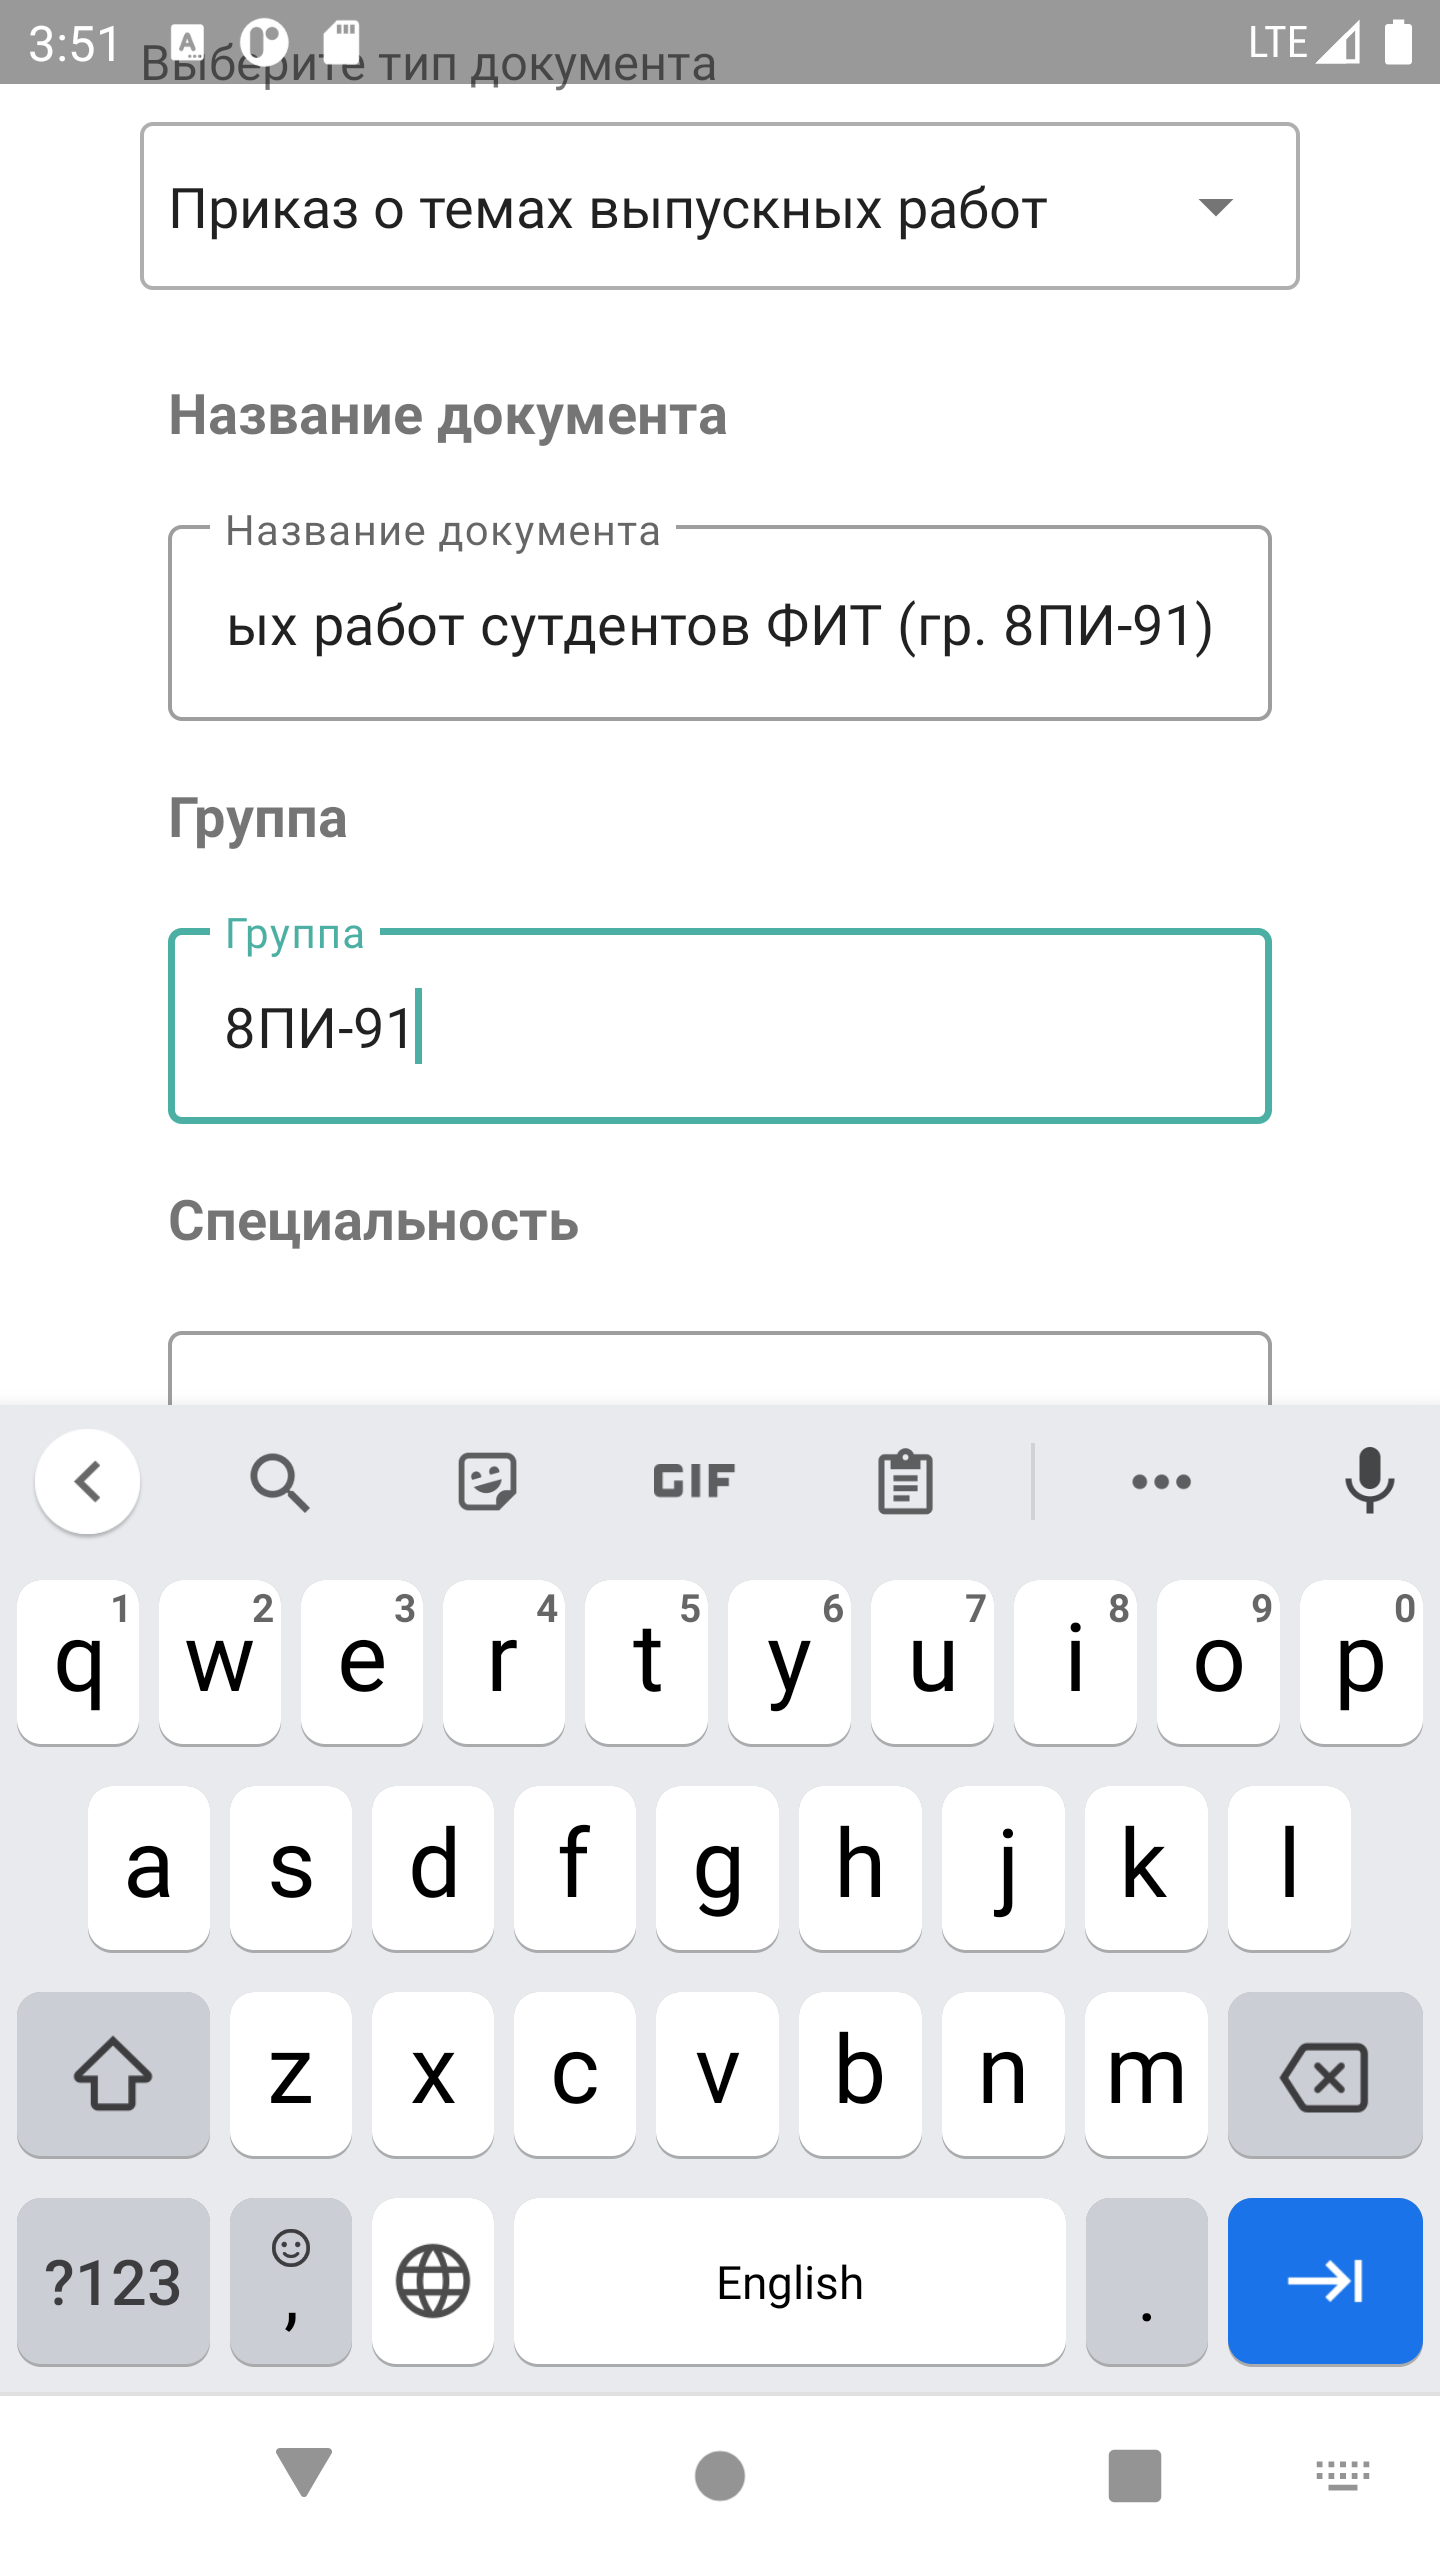
\includegraphics [scale=0.2] {doc-creating1}
	\caption{Создание документа типа <<Приказ о темах выпускных работ>>.}
	\label{fig:ui-first}
\end{figure}

\begin{figure}[ht]
	\centering
	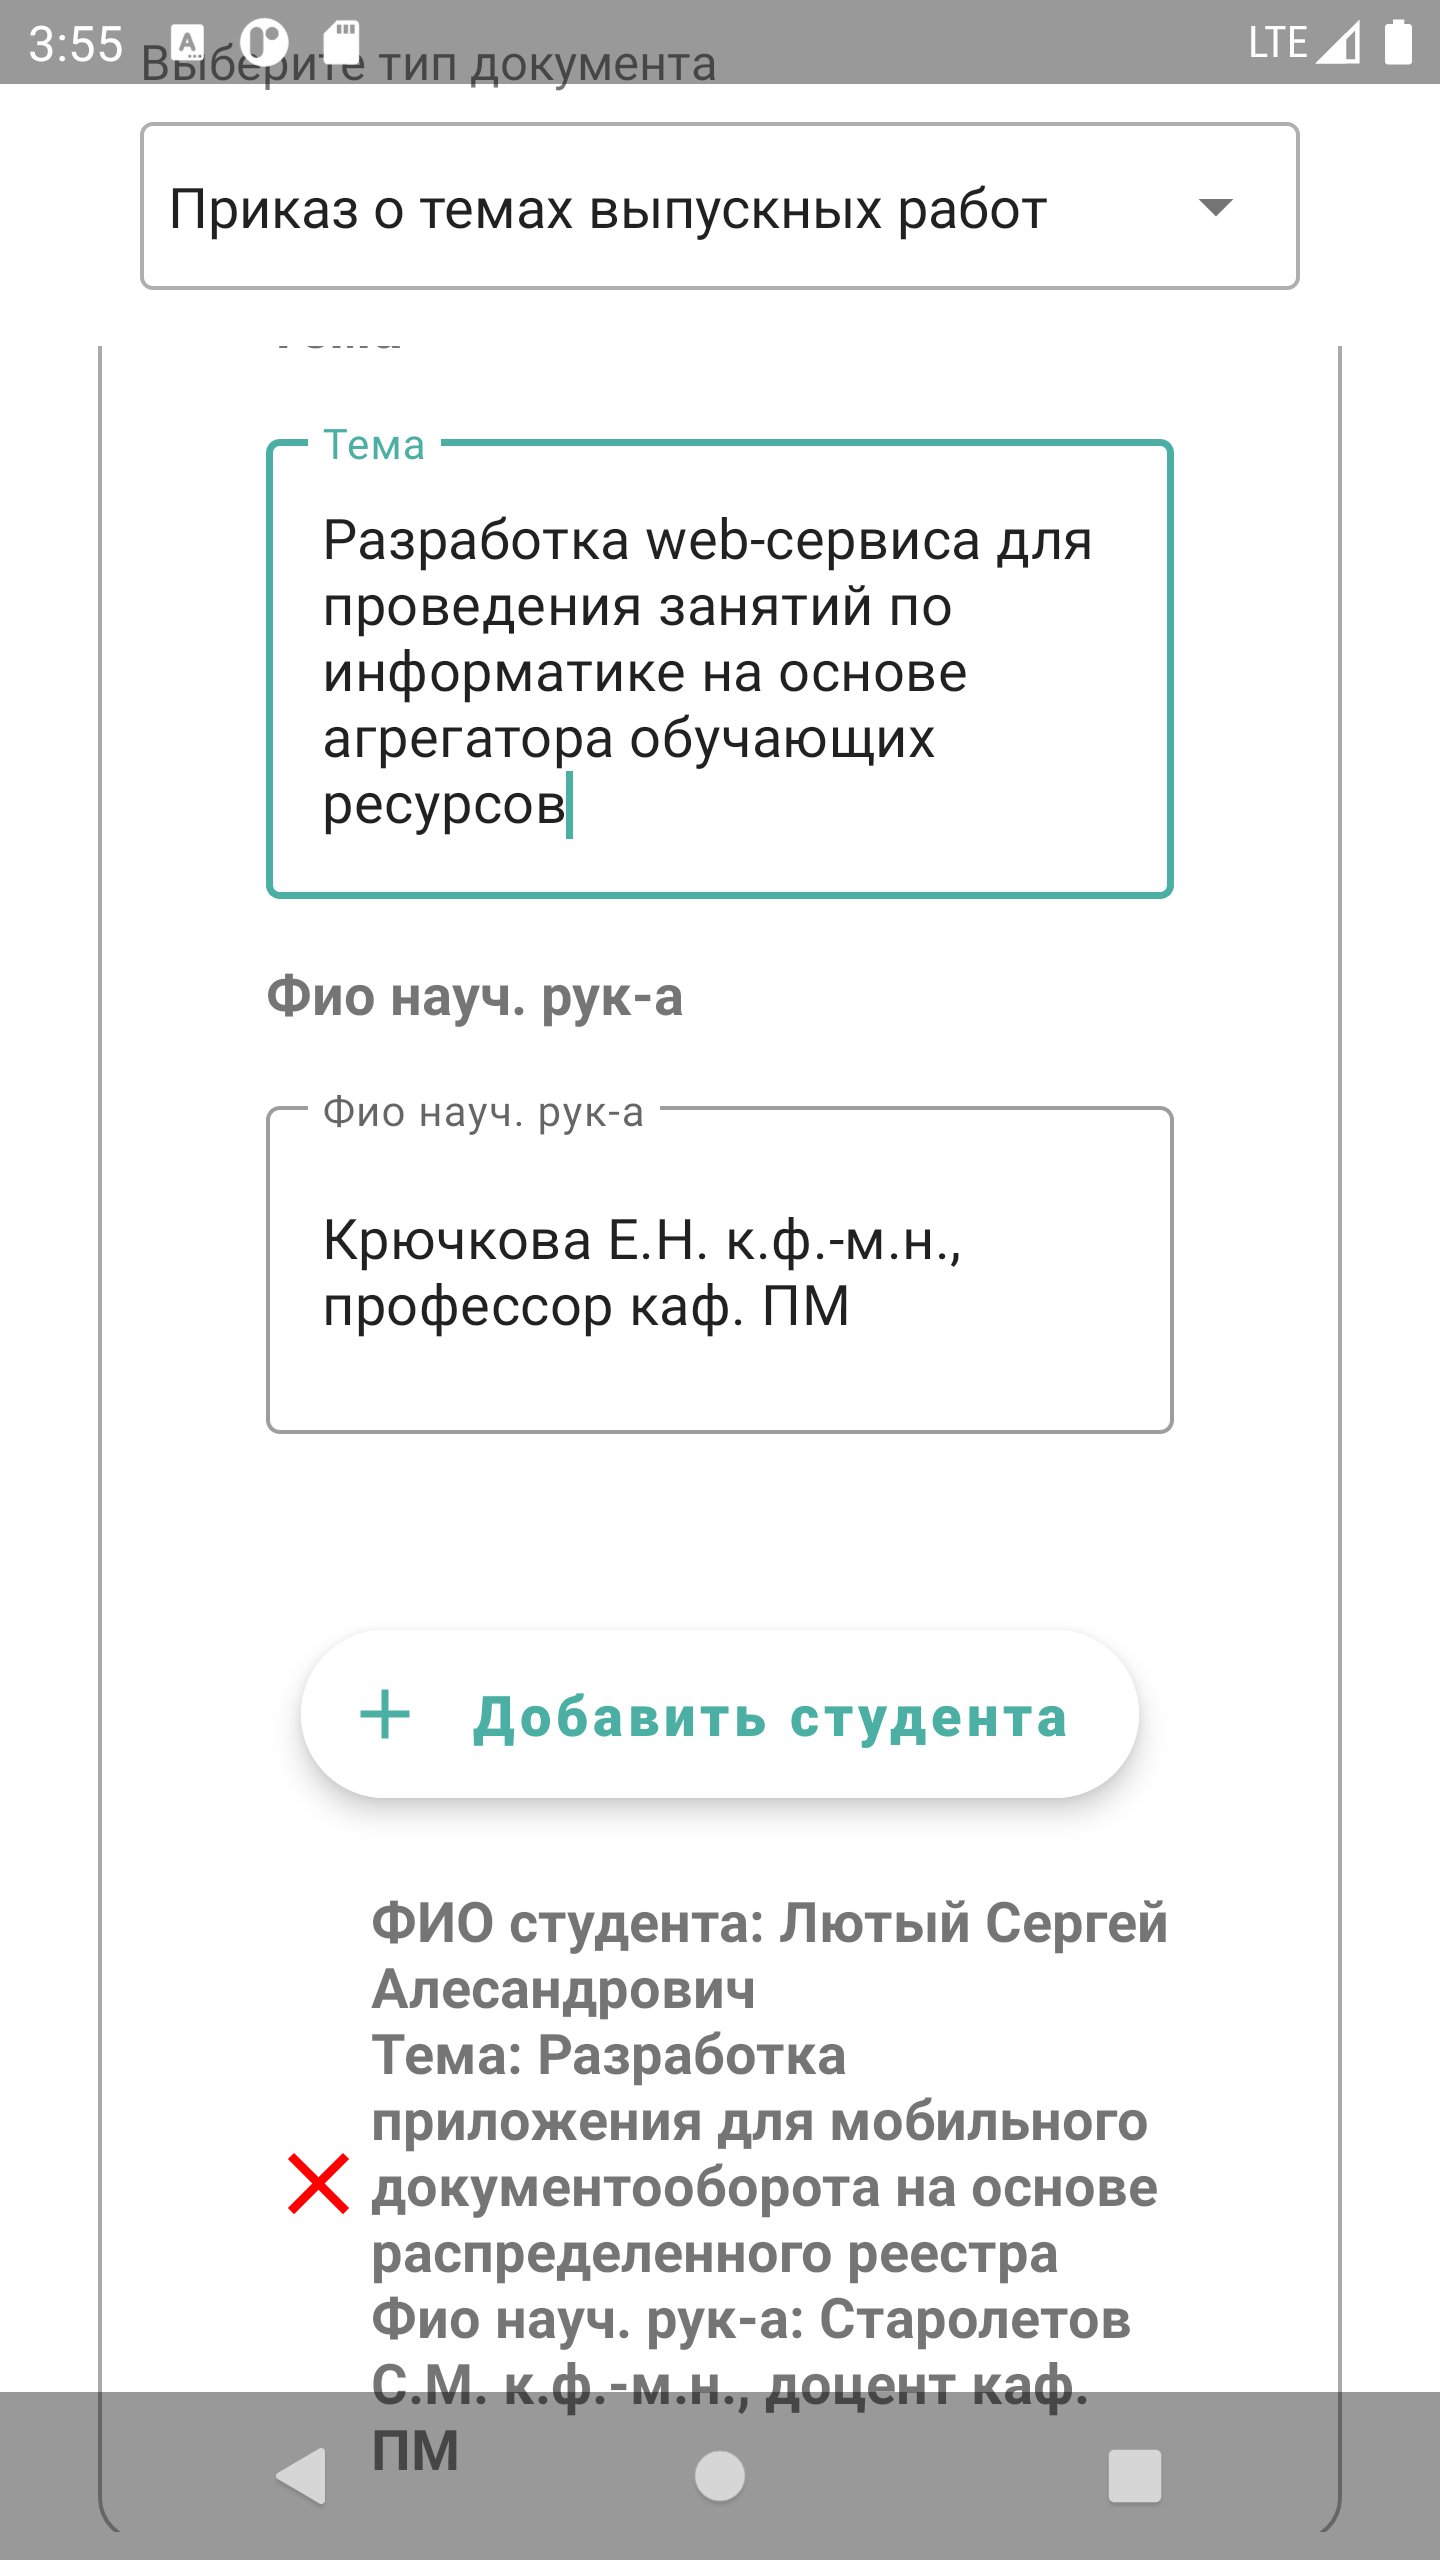
\includegraphics [scale=0.2] {doc-creating2}
	\caption{Добавление данных о студентах в создаваемый документ.}
	\label{fig:doc-creating2}
\end{figure}

\begin{figure}[ht]
	\centering
	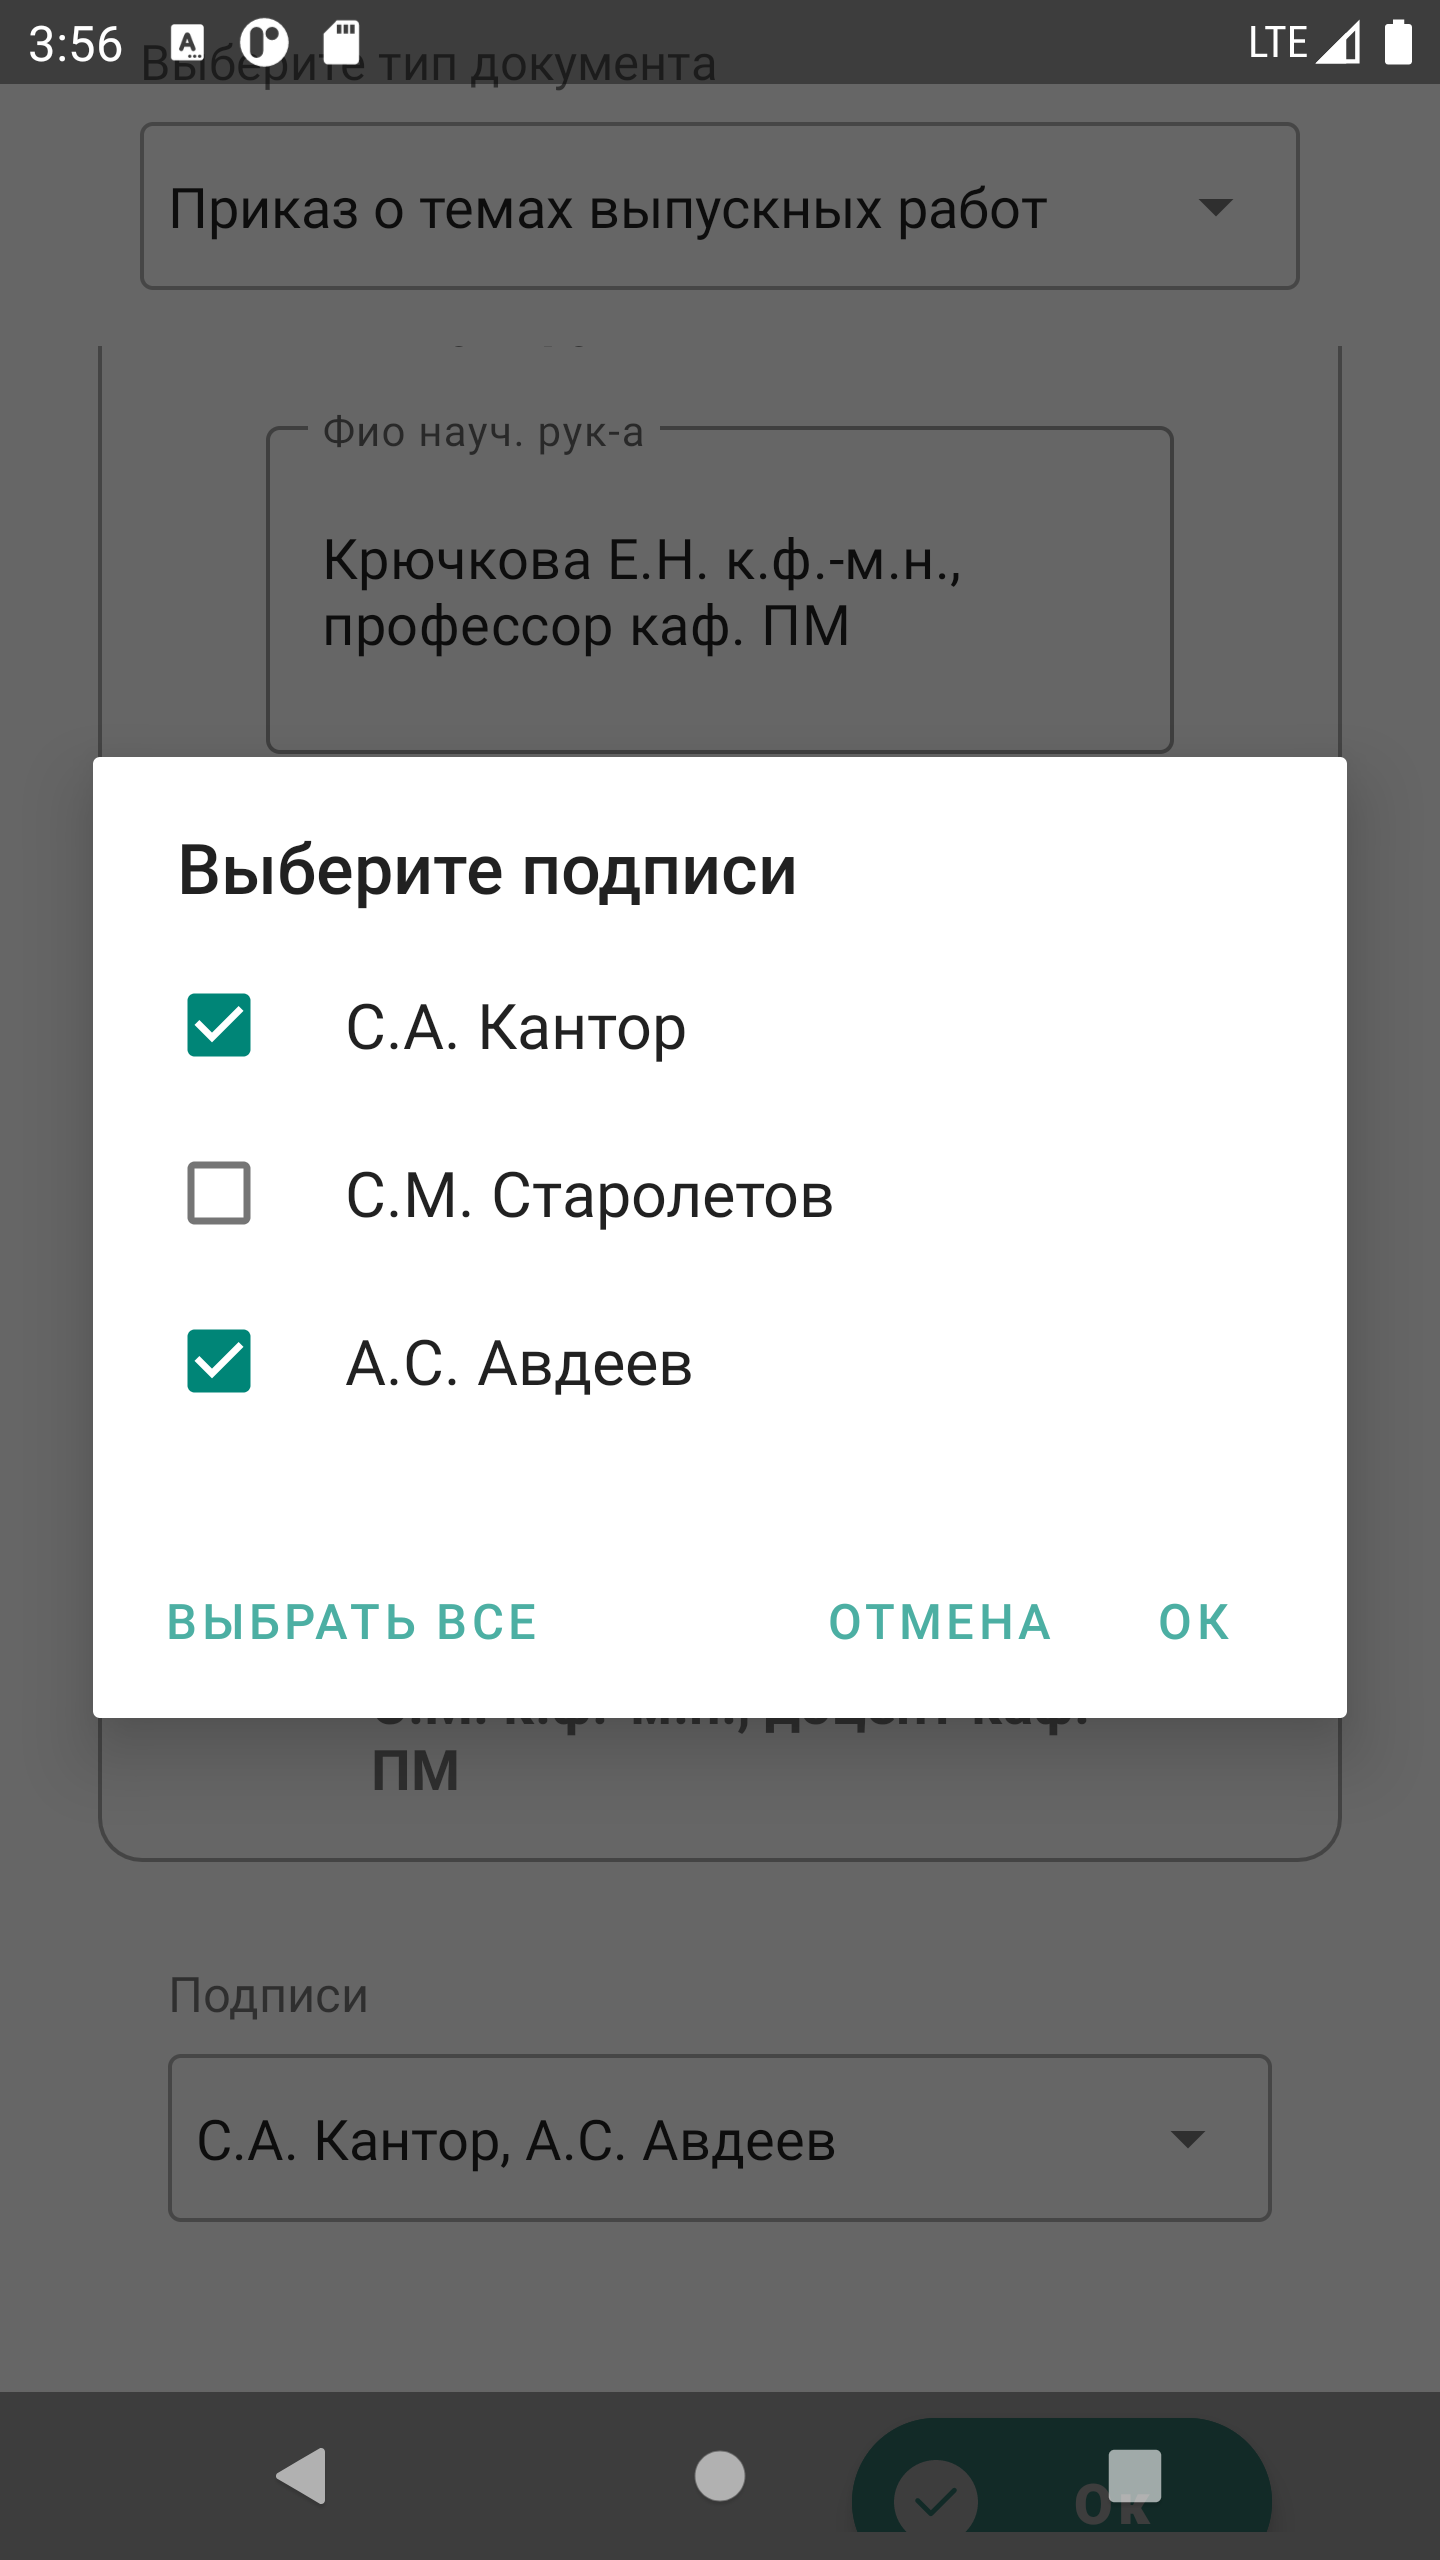
\includegraphics [scale=0.2] {doc-creating3}
	\caption{Указание необходимых подписантов.}
	\label{fig:doc-creating3}
\end{figure}

\begin{figure}[ht]
	\centering
	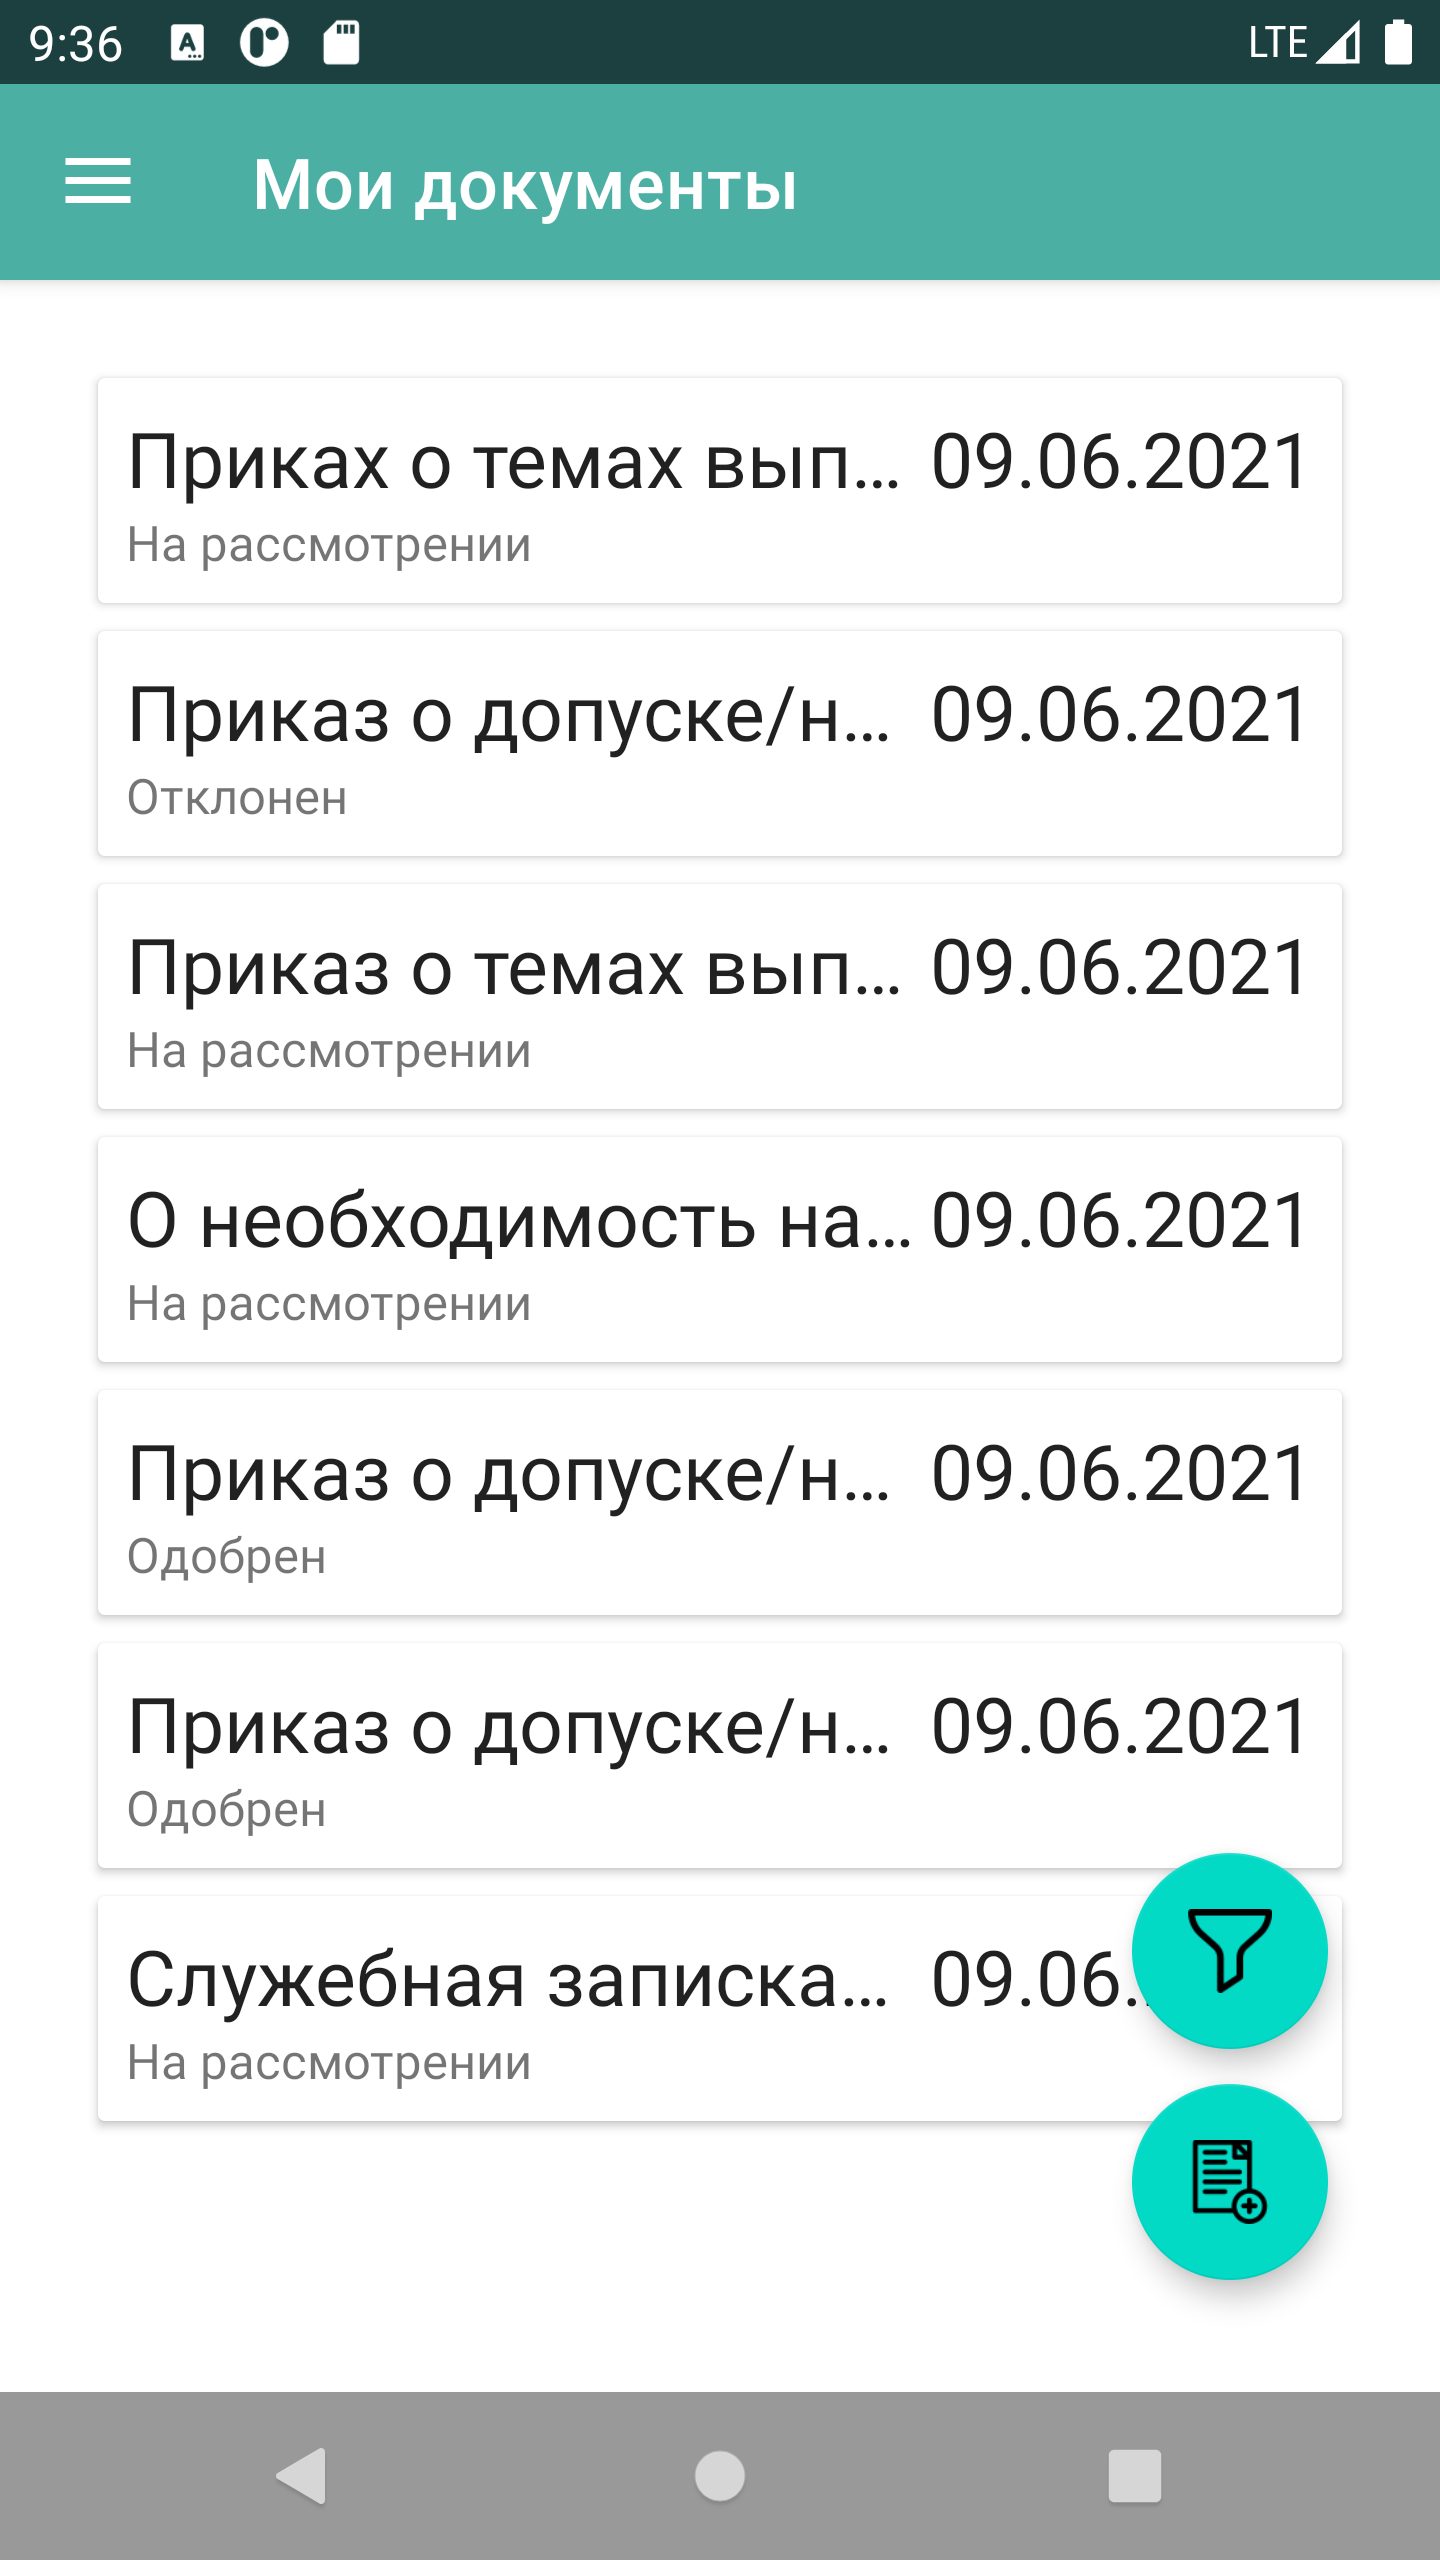
\includegraphics [scale=0.2] {before-filters}
	\caption{Список документов.}
	\label{fig:before-filters}
\end{figure}

\begin{figure}[ht]
	\centering
	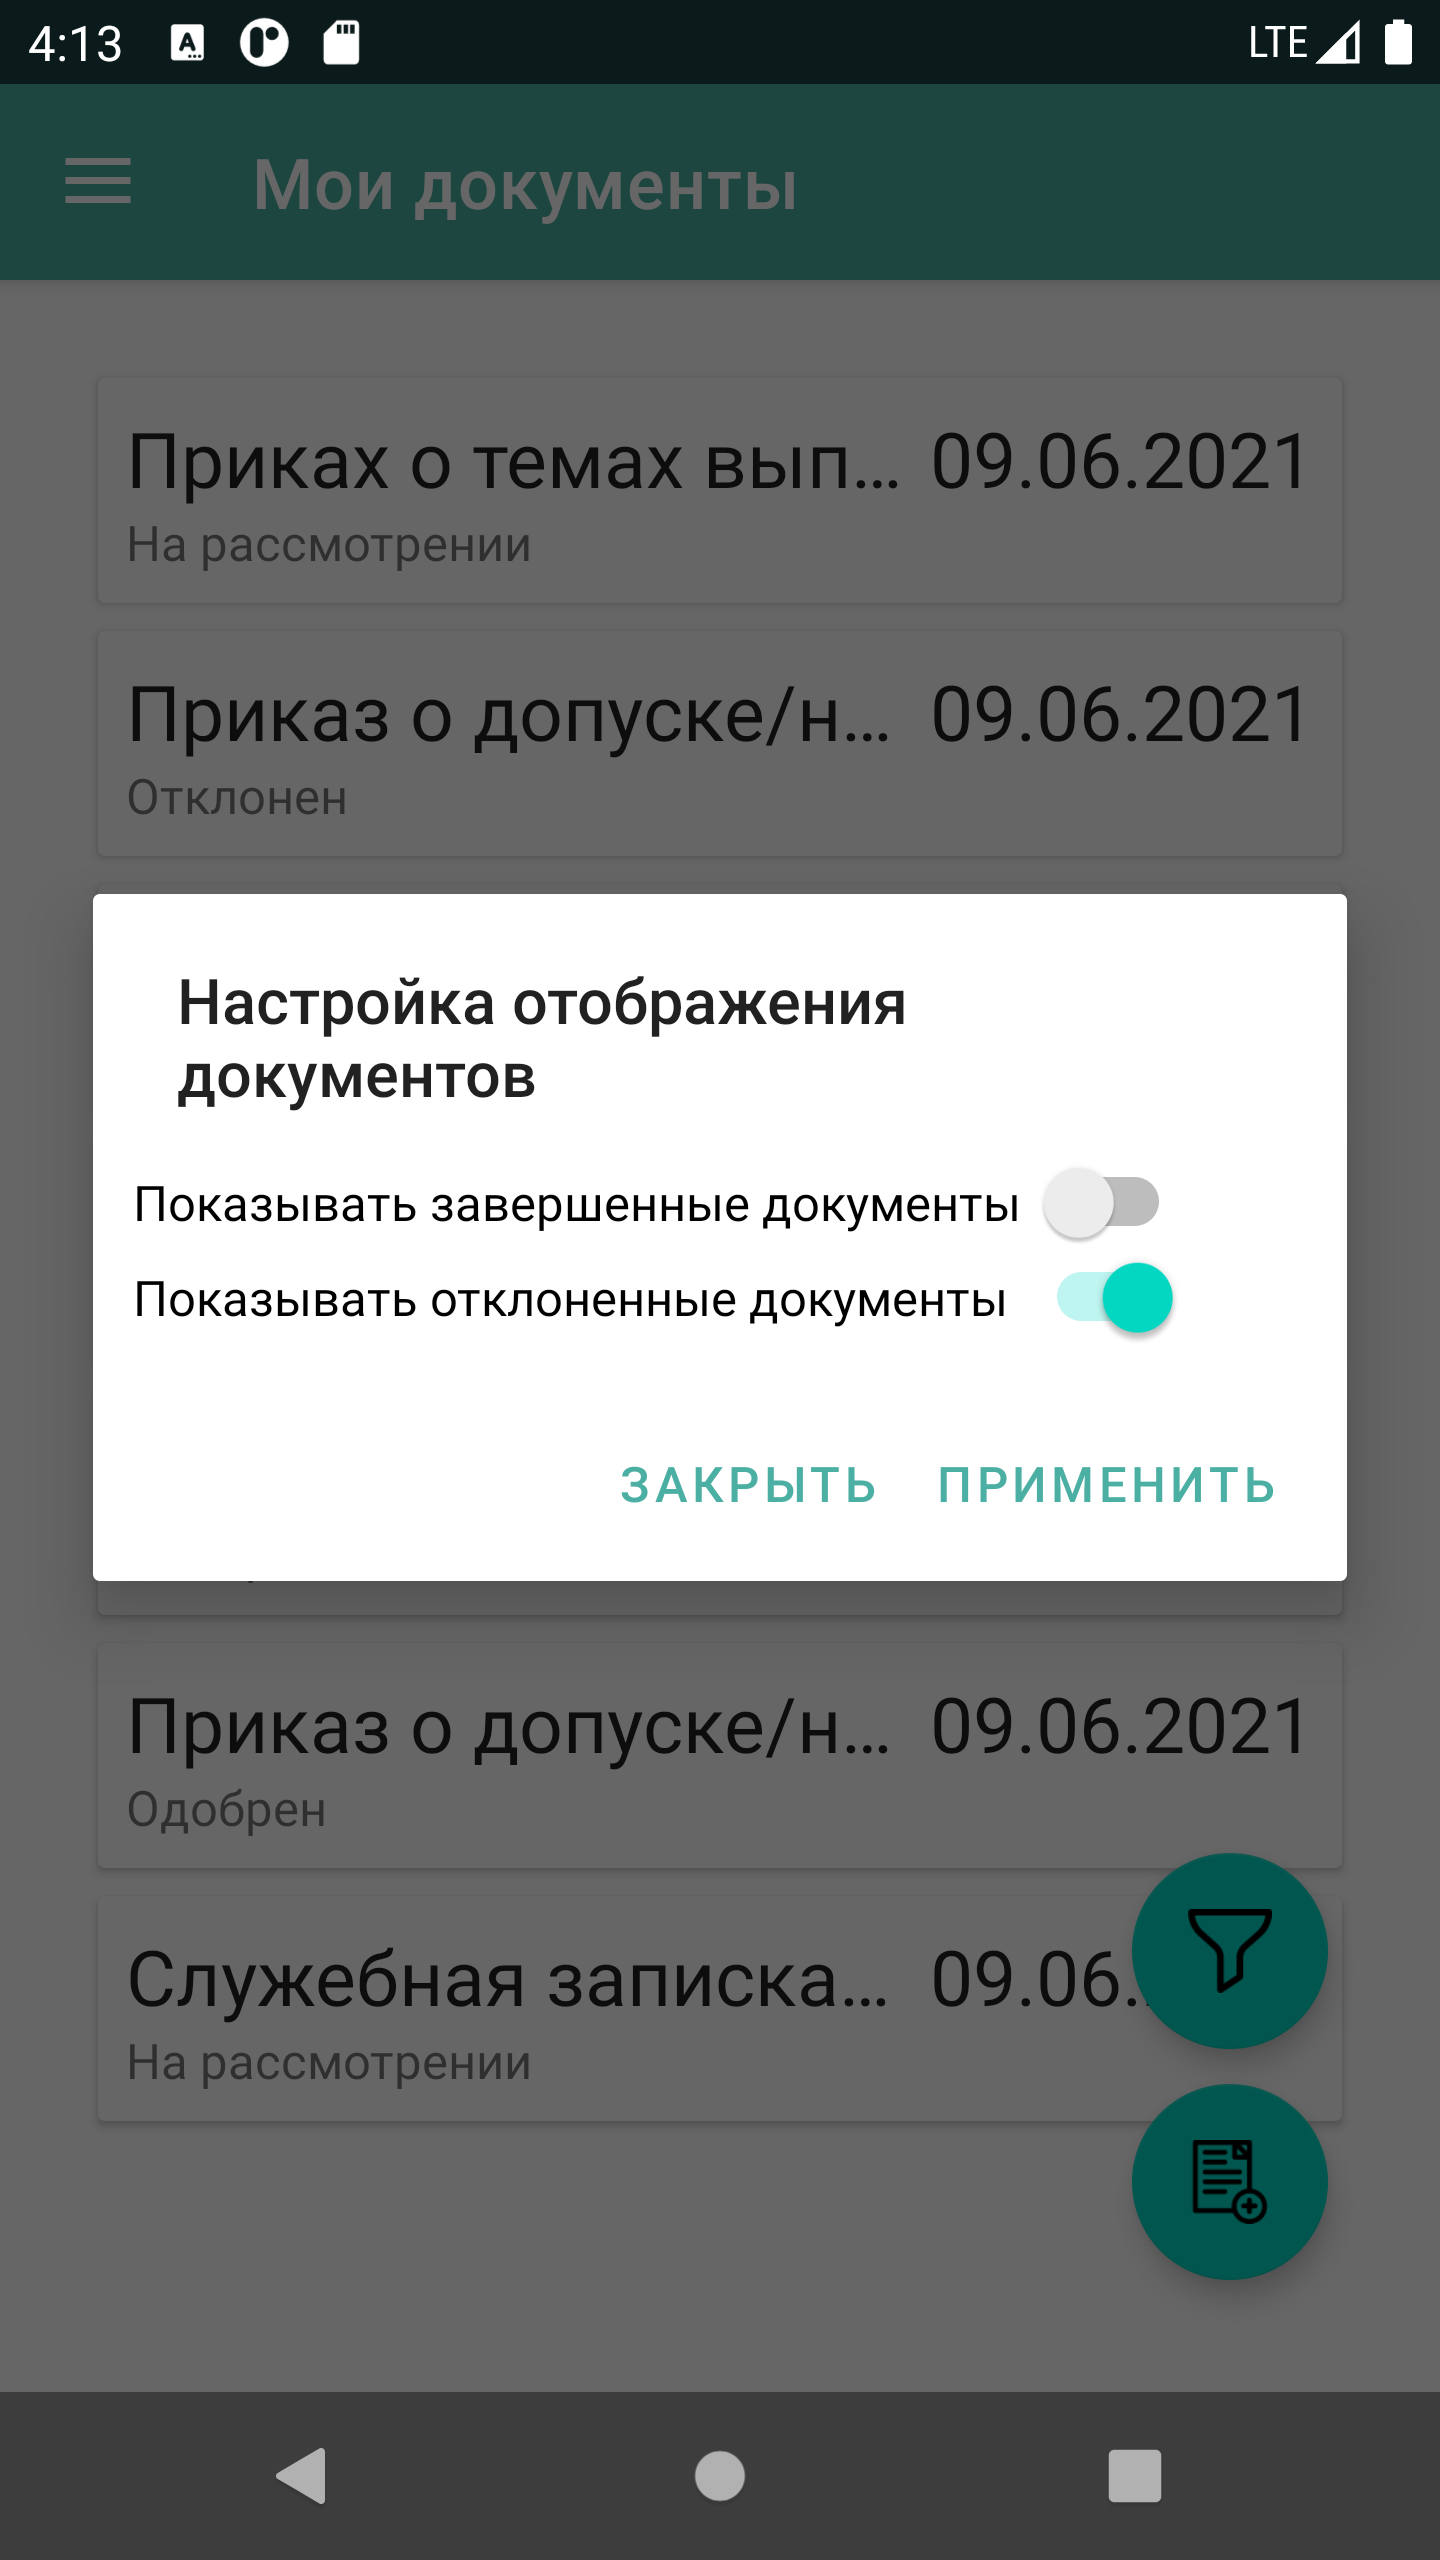
\includegraphics [scale=0.2] {filters}
	\caption{Настройка отображения списка документов.}
	\label{fig:filters}
\end{figure}

\begin{figure}[ht]
	\centering
	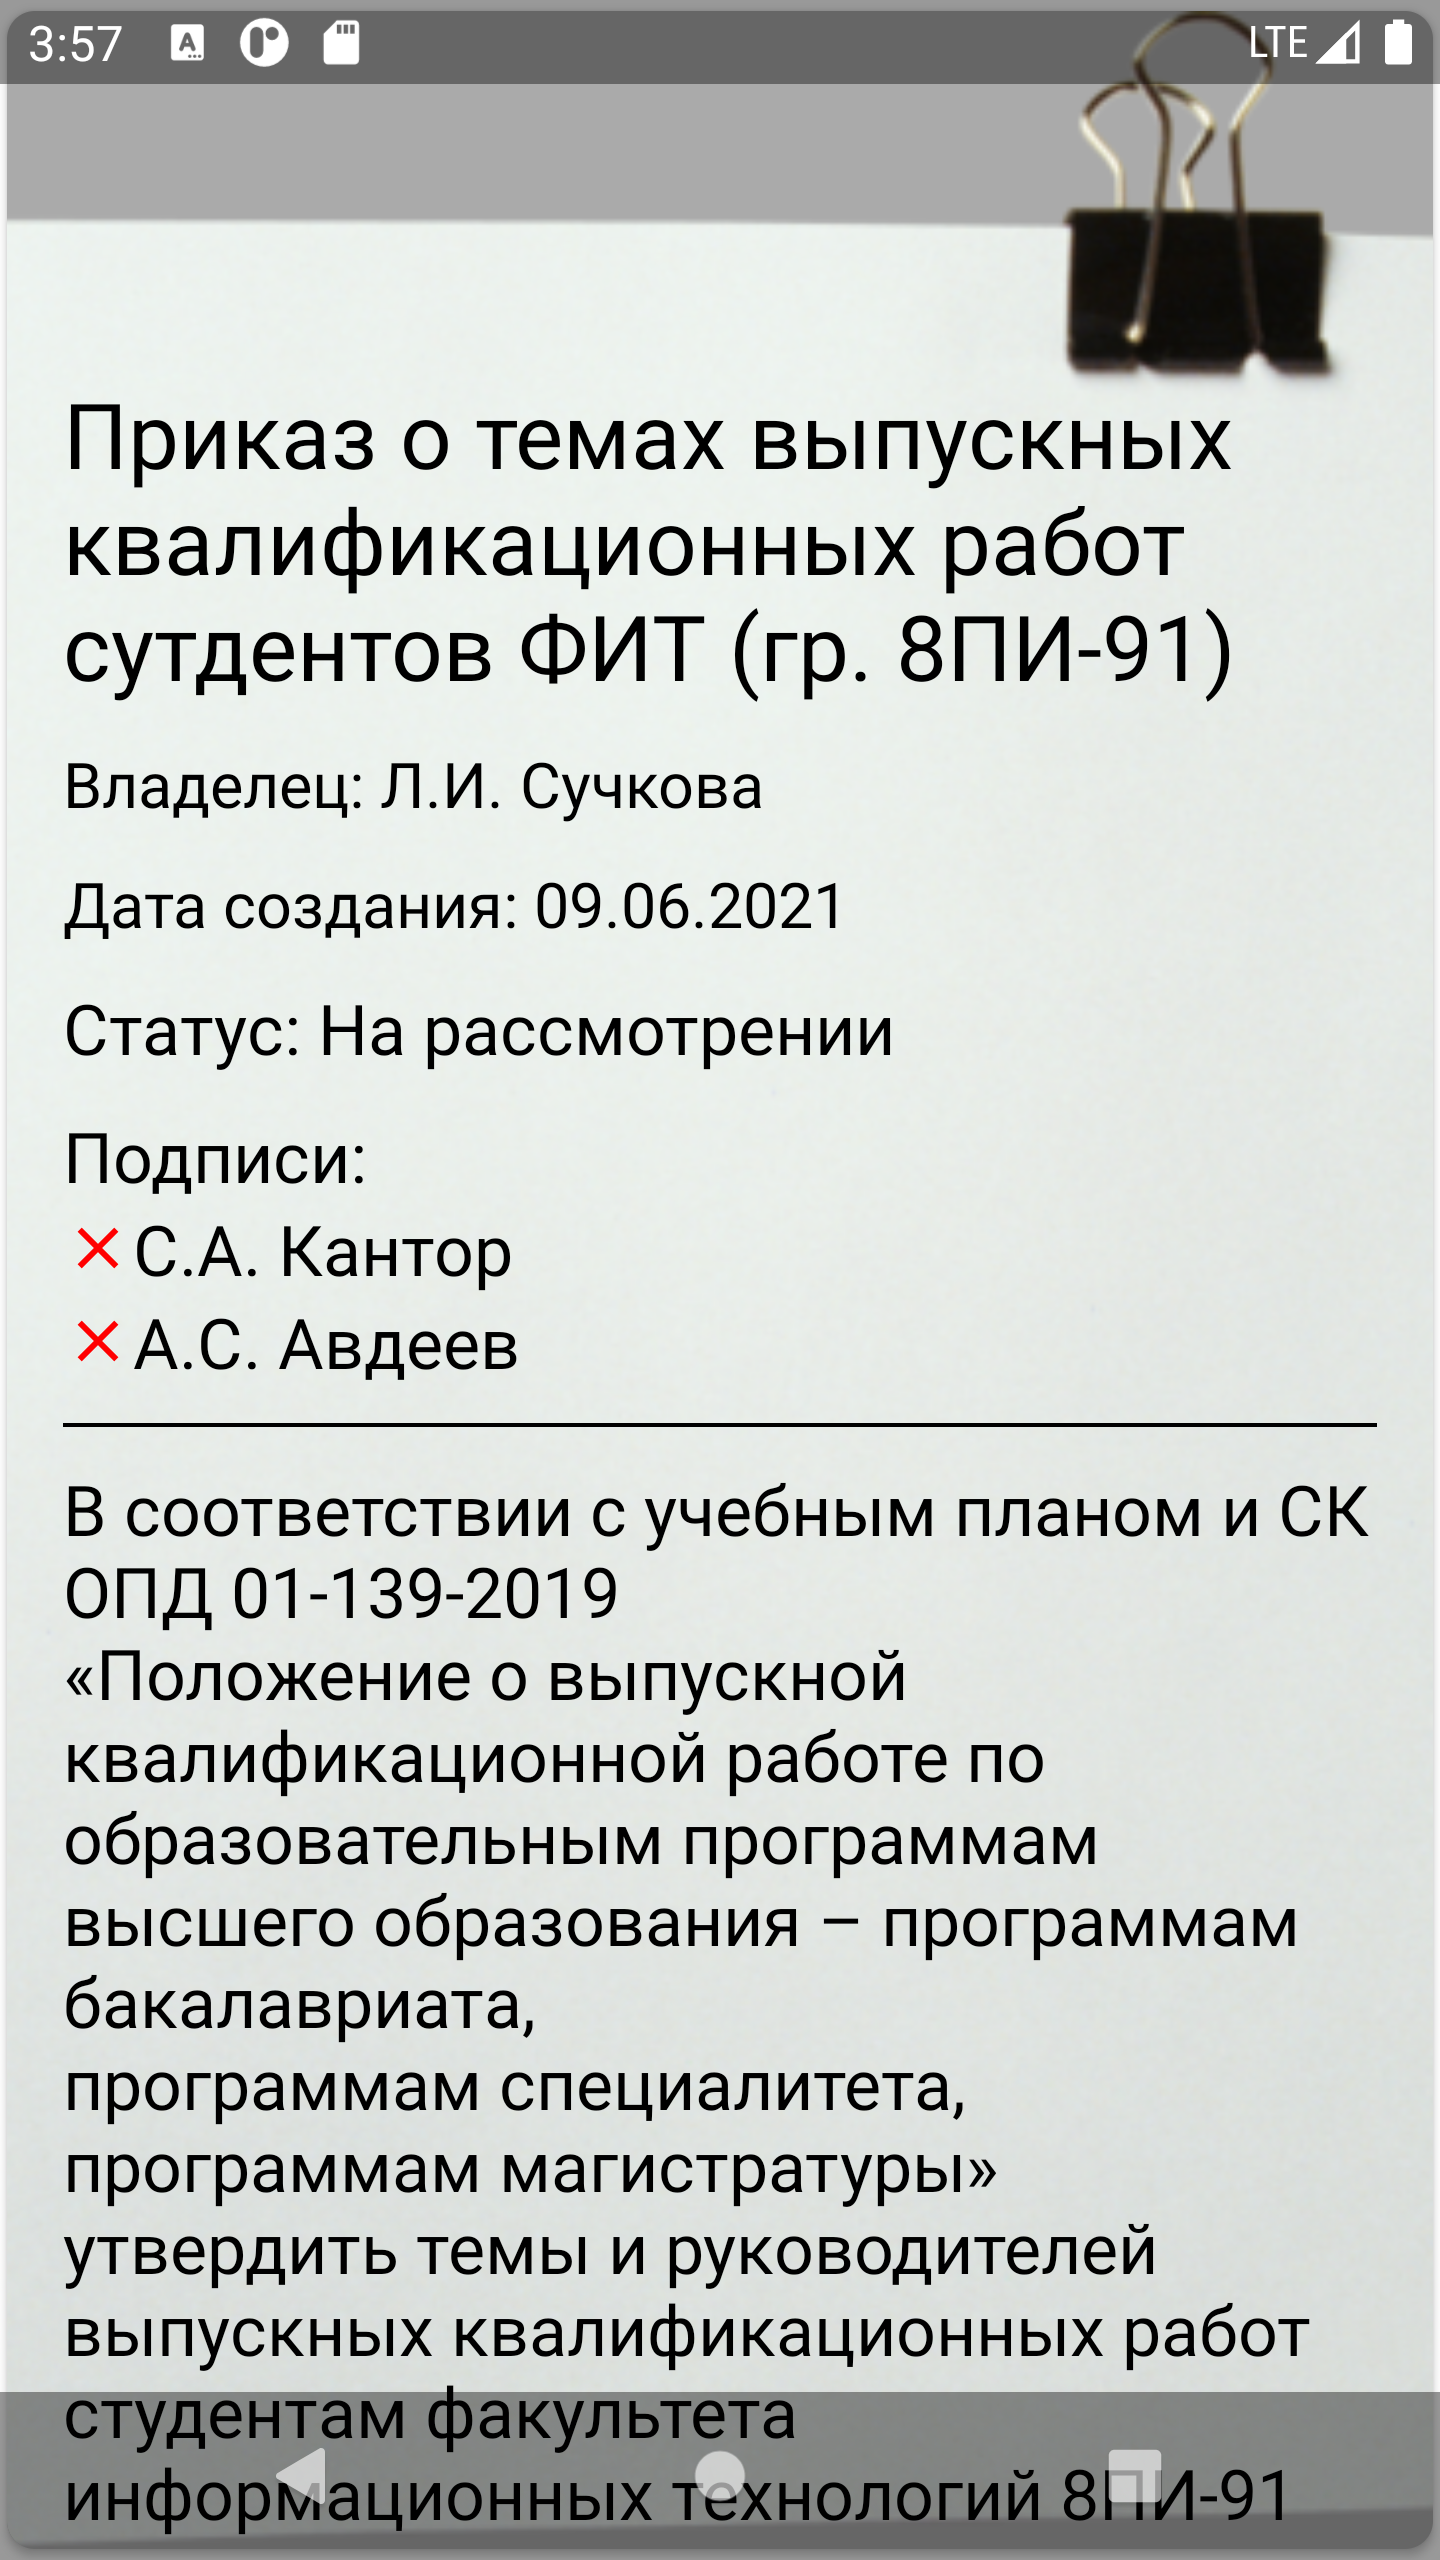
\includegraphics [scale=0.2] {doc-view}
	\caption{Просмотр деталей отдельного документа.}
	\label{fig:doc-view}
\end{figure}

\begin{figure}[ht]
	\centering
	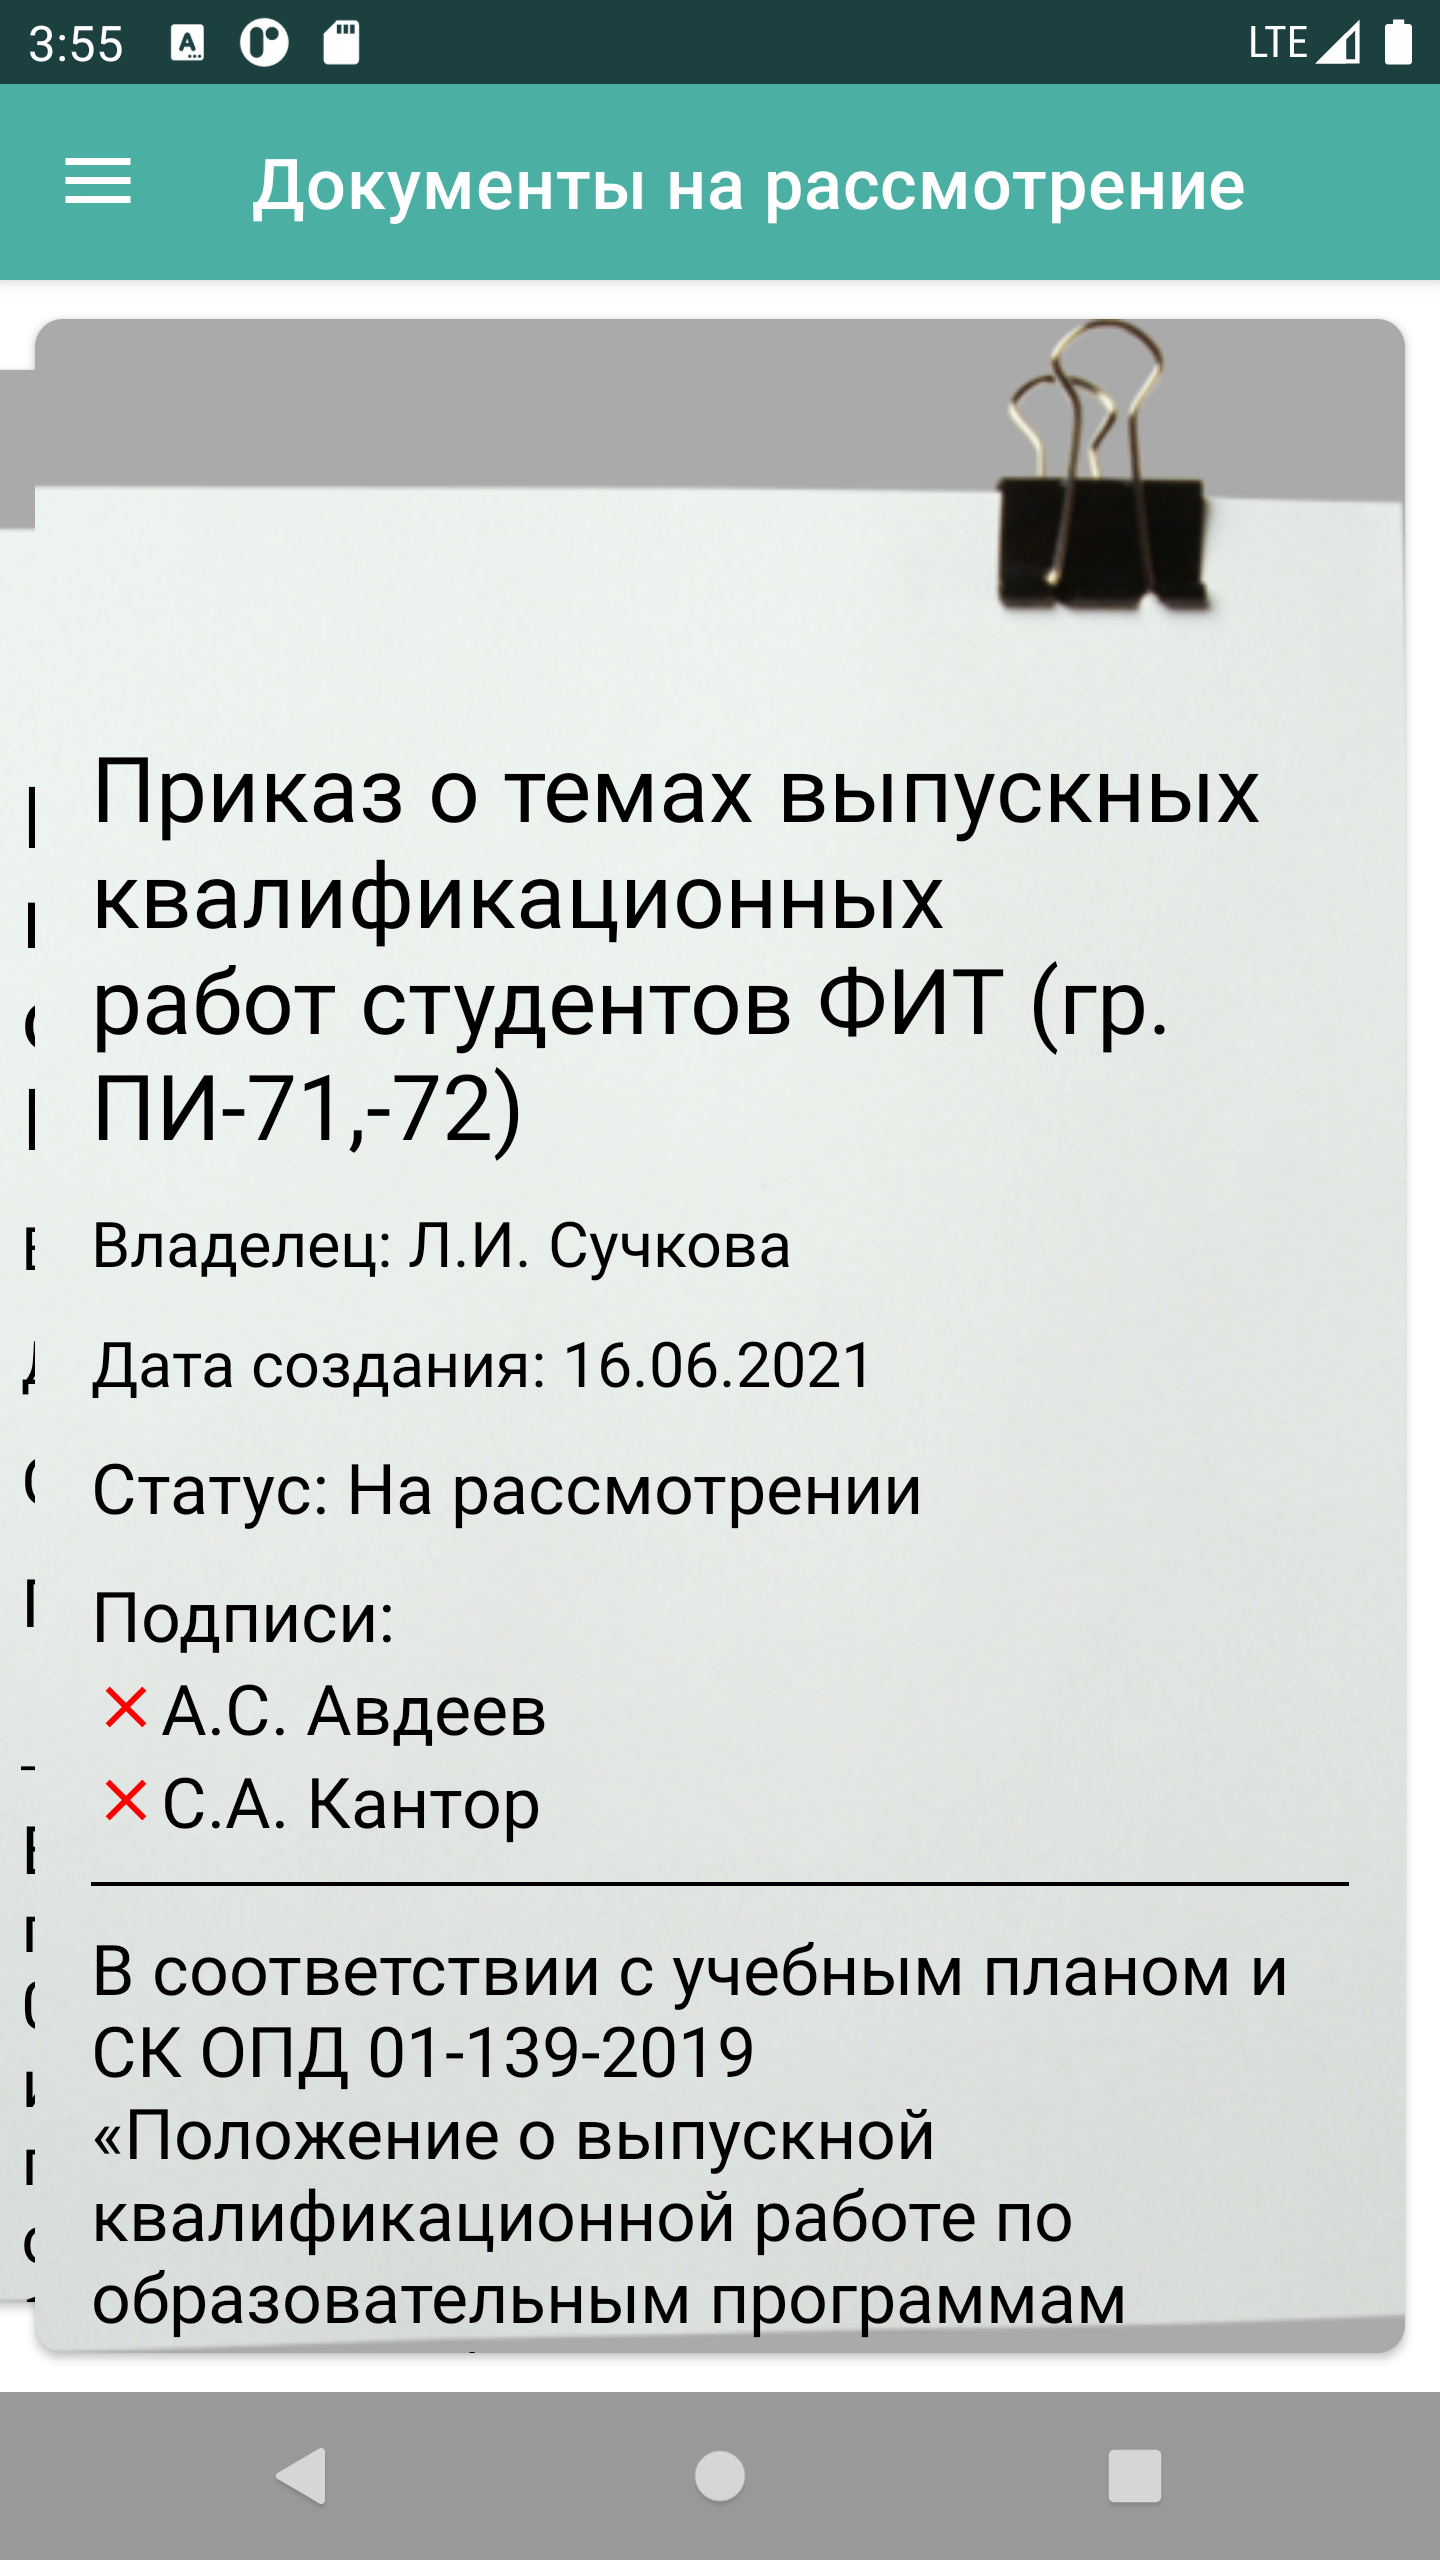
\includegraphics [scale=0.2] {doc-stack}
	\caption{Стопка документов на рассмотрение.}
	\label{fig:doc-stack}
\end{figure}

\begin{figure}[ht]
	\centering
	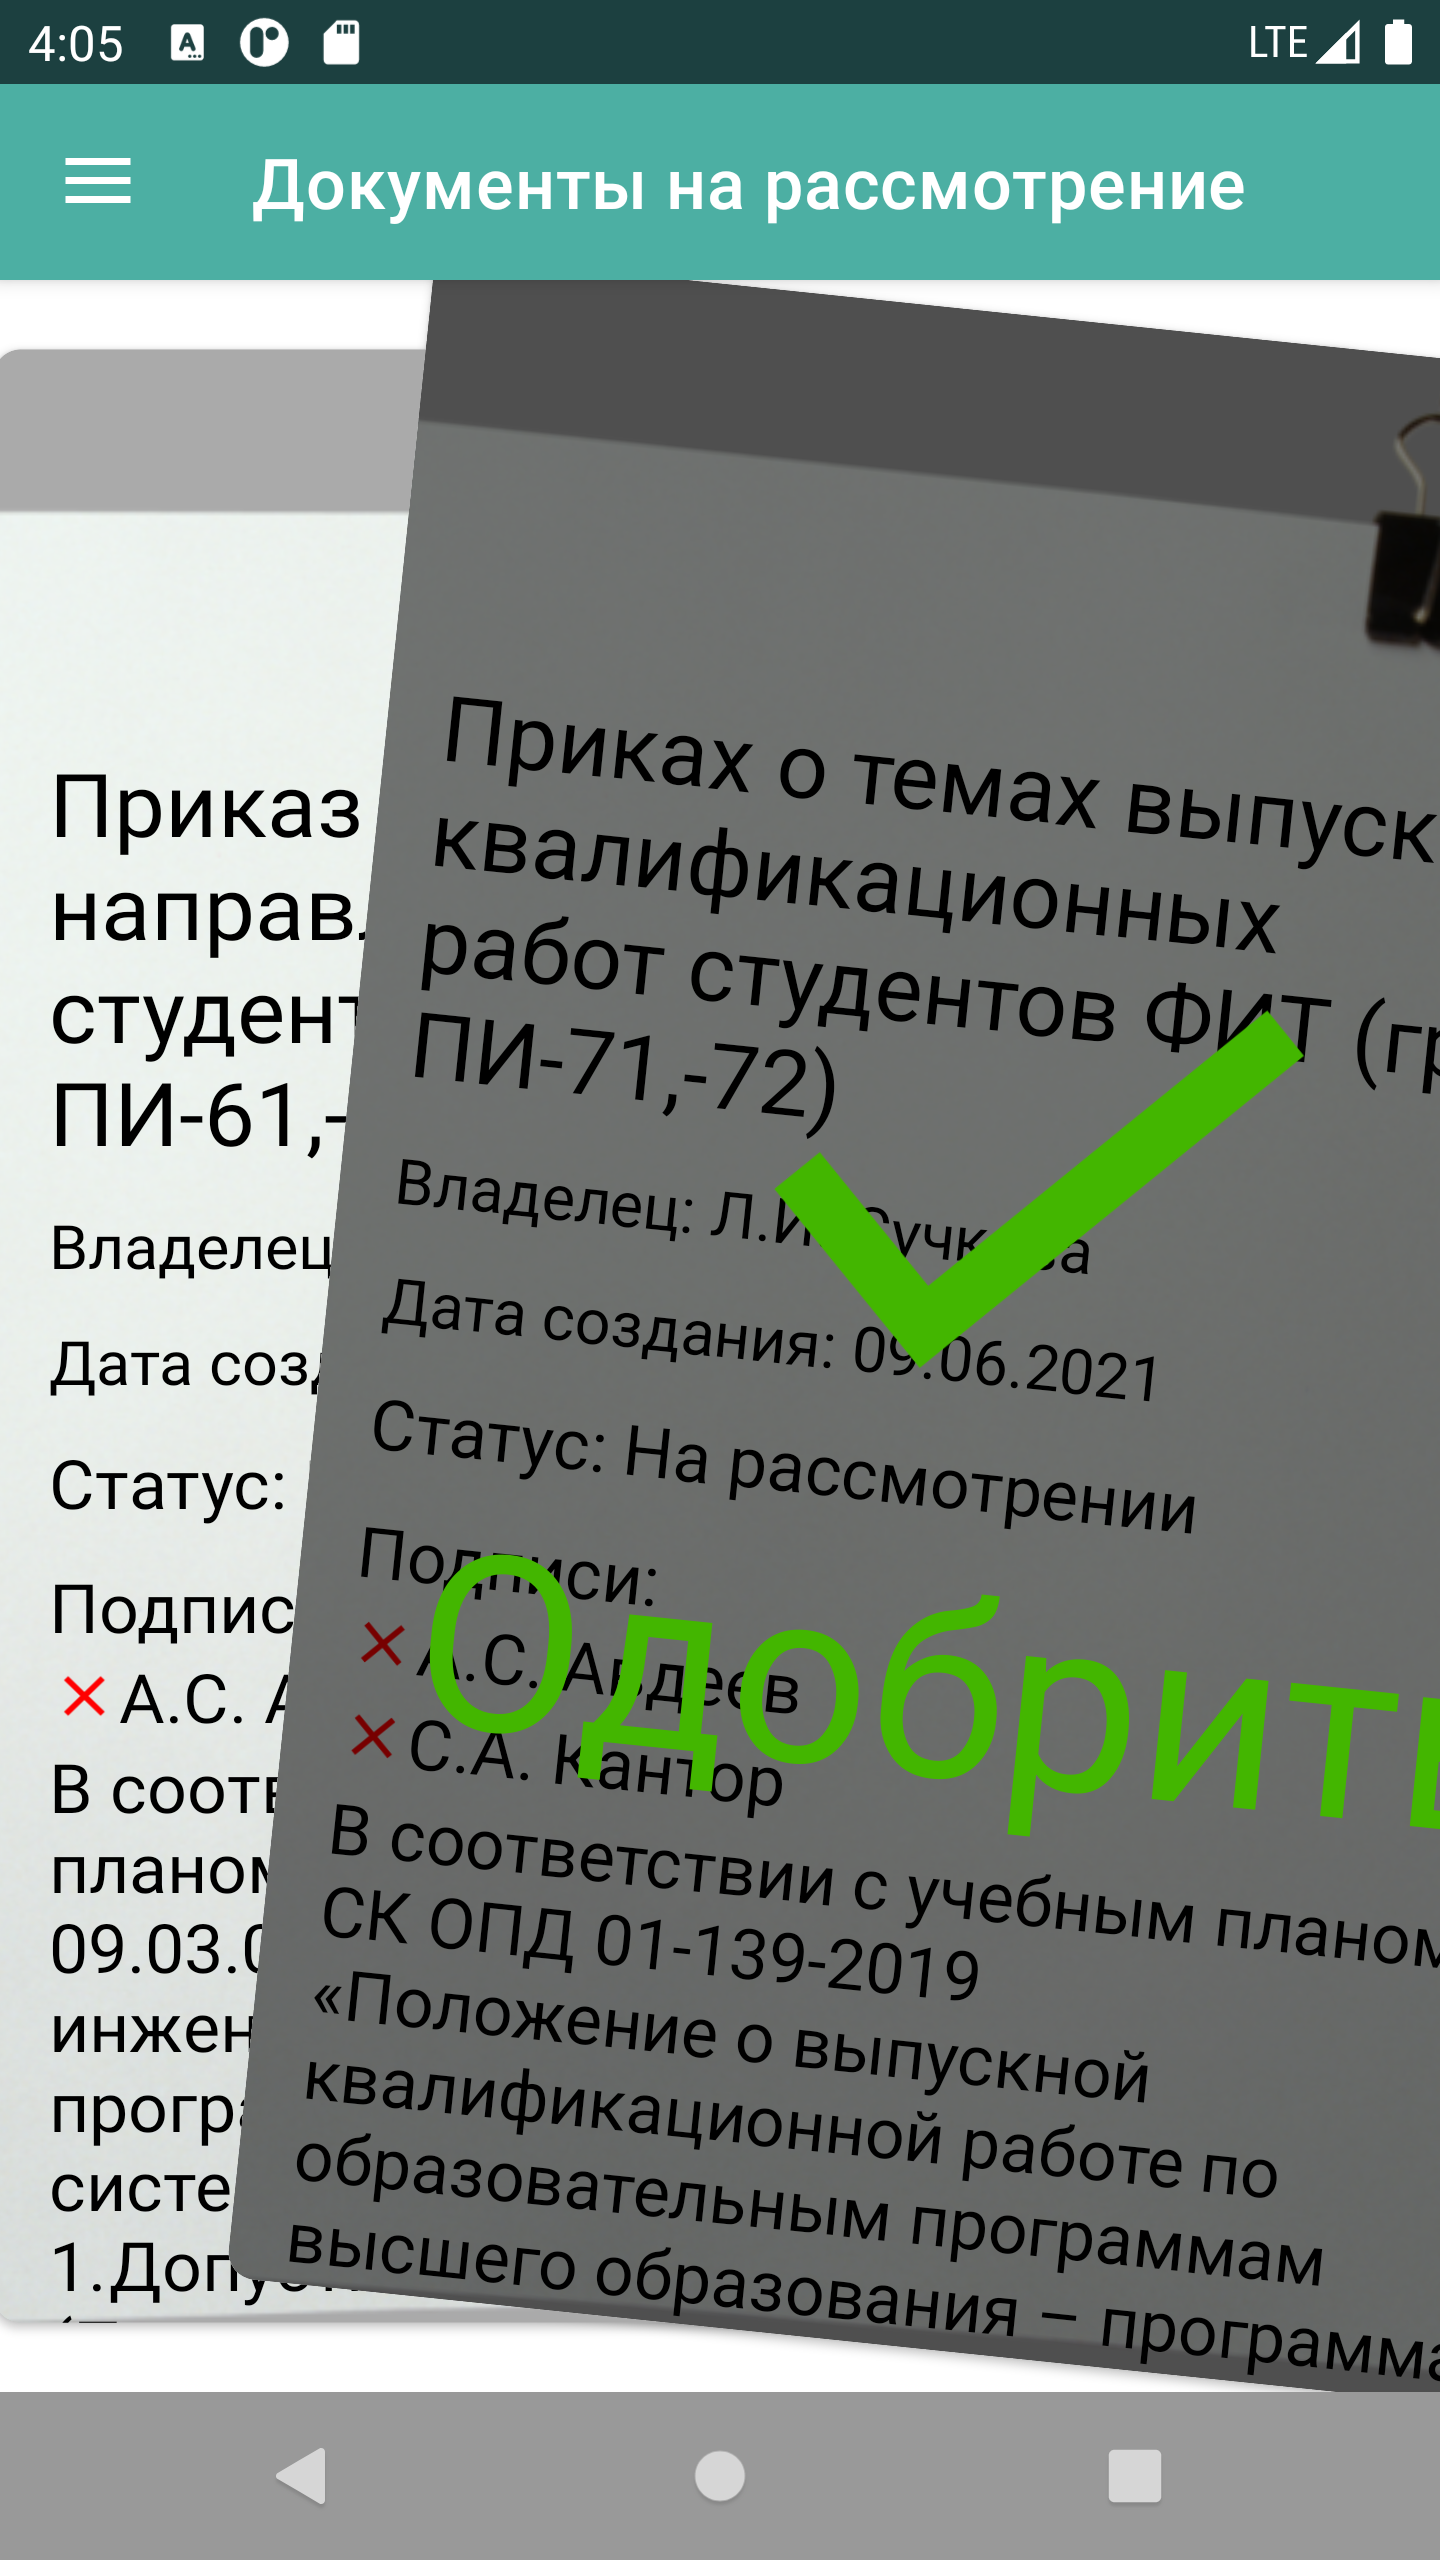
\includegraphics [scale=0.2] {approve}
	\caption{Одобрение (подписывание) документа.}
	\label{fig:approve}
\end{figure}

\begin{figure}[ht]
	\centering
	
\includegraphics [scale=0.2] {reject}
	\caption{Отклонение документа.}
	\label{fig:reject}
\end{figure}

\begin{figure}[ht]
	\centering
	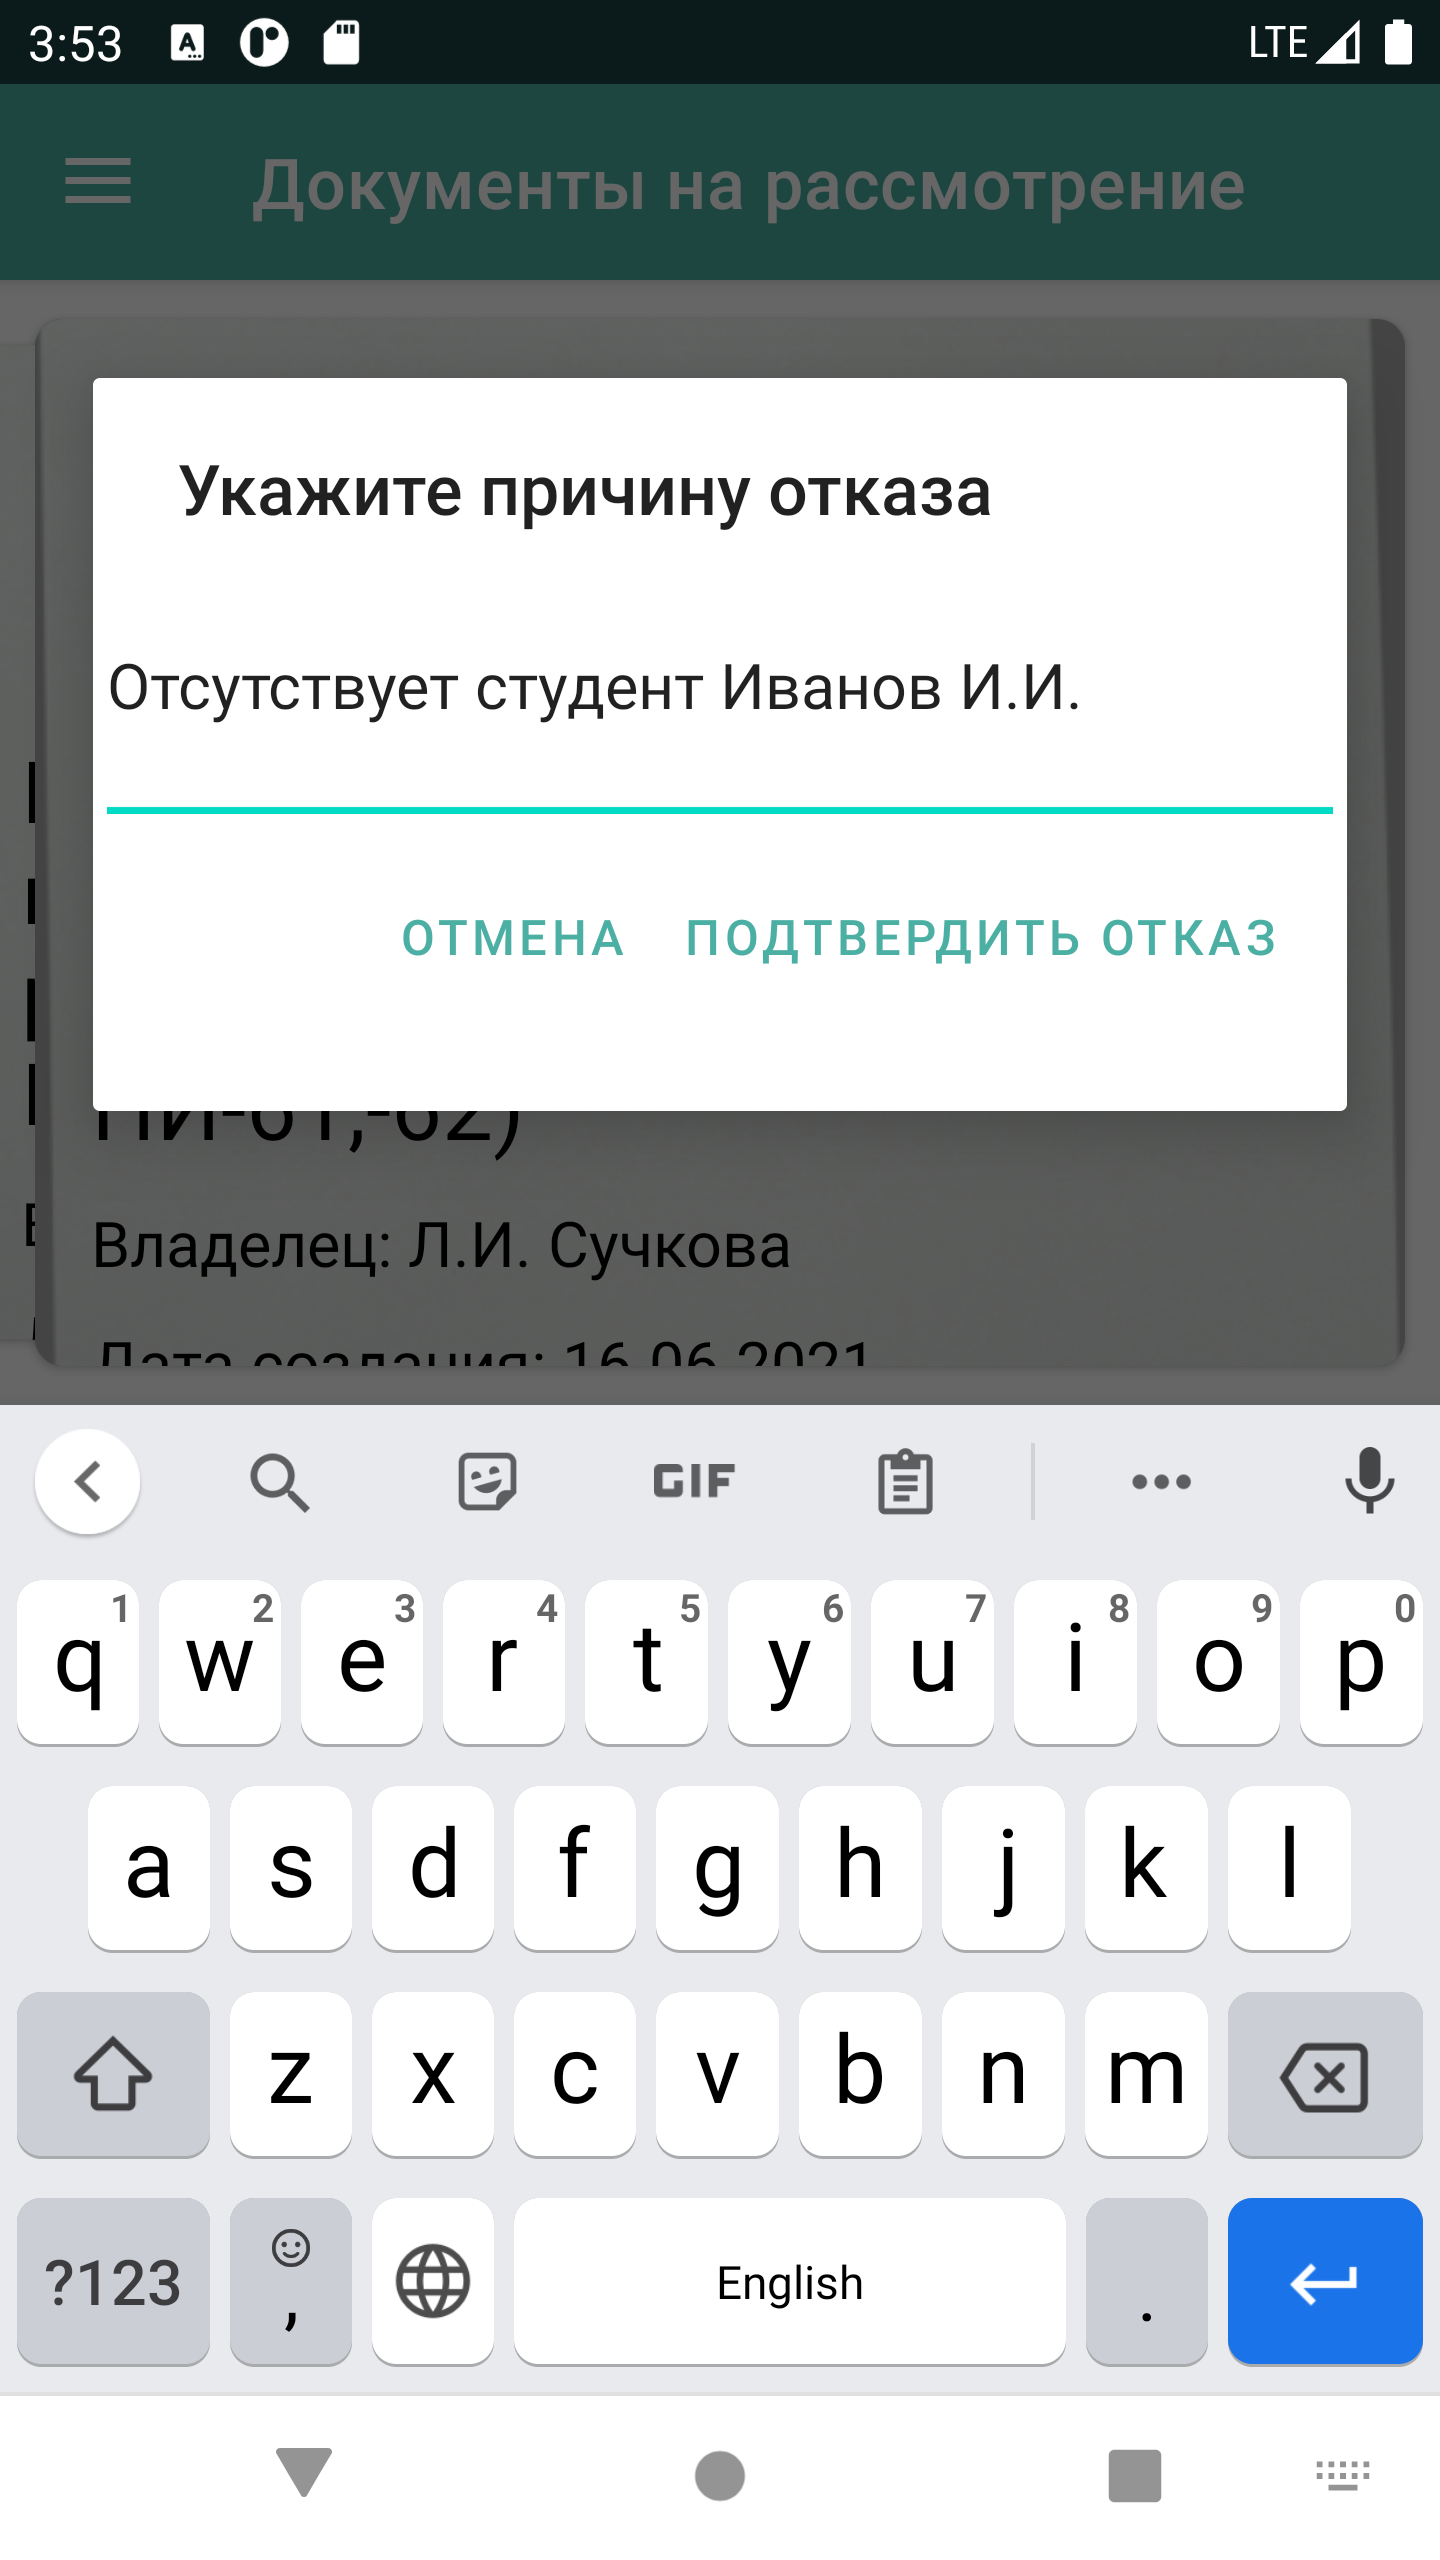
\includegraphics [scale=0.2] {reason-for-reject}
	\caption{Указание причины отказа в качестве комментария.}
	\label{fig:ui-last}
\end{figure}